\documentclass[11pt]{article}

    \usepackage[breakable]{tcolorbox}
    \usepackage{parskip} % Stop auto-indenting (to mimic markdown behaviour)
    
    \usepackage{iftex}
    \ifPDFTeX
    	\usepackage[T1]{fontenc}
    	\usepackage{mathpazo}
    \else
    	\usepackage{fontspec}
    \fi

    % Basic figure setup, for now with no caption control since it's done
    % automatically by Pandoc (which extracts ![](path) syntax from Markdown).
    \usepackage{graphicx}
    % Maintain compatibility with old templates. Remove in nbconvert 6.0
    \let\Oldincludegraphics\includegraphics
    % Ensure that by default, figures have no caption (until we provide a
    % proper Figure object with a Caption API and a way to capture that
    % in the conversion process - todo).
    \usepackage{caption}
    \DeclareCaptionFormat{nocaption}{}
    \captionsetup{format=nocaption,aboveskip=0pt,belowskip=0pt}

    \usepackage{float}
    \floatplacement{figure}{H} % forces figures to be placed at the correct location
    \usepackage{xcolor} % Allow colors to be defined
    \usepackage{enumerate} % Needed for markdown enumerations to work
    \usepackage{geometry} % Used to adjust the document margins
    \usepackage{amsmath} % Equations
    \usepackage{amssymb} % Equations
    \usepackage{textcomp} % defines textquotesingle
    % Hack from http://tex.stackexchange.com/a/47451/13684:
    \AtBeginDocument{%
        \def\PYZsq{\textquotesingle}% Upright quotes in Pygmentized code
    }
    \usepackage{upquote} % Upright quotes for verbatim code
    \usepackage{eurosym} % defines \euro
    \usepackage[mathletters]{ucs} % Extended unicode (utf-8) support
    \usepackage{fancyvrb} % verbatim replacement that allows latex
    \usepackage{grffile} % extends the file name processing of package graphics 
                         % to support a larger range
    \makeatletter % fix for old versions of grffile with XeLaTeX
    \@ifpackagelater{grffile}{2019/11/01}
    {
      % Do nothing on new versions
    }
    {
      \def\Gread@@xetex#1{%
        \IfFileExists{"\Gin@base".bb}%
        {\Gread@eps{\Gin@base.bb}}%
        {\Gread@@xetex@aux#1}%
      }
    }
    \makeatother
    \usepackage[Export]{adjustbox} % Used to constrain images to a maximum size
    \adjustboxset{max size={0.9\linewidth}{0.9\paperheight}}

    % The hyperref package gives us a pdf with properly built
    % internal navigation ('pdf bookmarks' for the table of contents,
    % internal cross-reference links, web links for URLs, etc.)
    \usepackage{hyperref}
    % The default LaTeX title has an obnoxious amount of whitespace. By default,
    % titling removes some of it. It also provides customization options.
    \usepackage{titling}
    \usepackage{longtable} % longtable support required by pandoc >1.10
    \usepackage{booktabs}  % table support for pandoc > 1.12.2
    \usepackage[inline]{enumitem} % IRkernel/repr support (it uses the enumerate* environment)
    \usepackage[normalem]{ulem} % ulem is needed to support strikethroughs (\sout)
                                % normalem makes italics be italics, not underlines
    \usepackage{mathrsfs}
    

    
    % Colors for the hyperref package
    \definecolor{urlcolor}{rgb}{0,.145,.698}
    \definecolor{linkcolor}{rgb}{.71,0.21,0.01}
    \definecolor{citecolor}{rgb}{.12,.54,.11}

    % ANSI colors
    \definecolor{ansi-black}{HTML}{3E424D}
    \definecolor{ansi-black-intense}{HTML}{282C36}
    \definecolor{ansi-red}{HTML}{E75C58}
    \definecolor{ansi-red-intense}{HTML}{B22B31}
    \definecolor{ansi-green}{HTML}{00A250}
    \definecolor{ansi-green-intense}{HTML}{007427}
    \definecolor{ansi-yellow}{HTML}{DDB62B}
    \definecolor{ansi-yellow-intense}{HTML}{B27D12}
    \definecolor{ansi-blue}{HTML}{208FFB}
    \definecolor{ansi-blue-intense}{HTML}{0065CA}
    \definecolor{ansi-magenta}{HTML}{D160C4}
    \definecolor{ansi-magenta-intense}{HTML}{A03196}
    \definecolor{ansi-cyan}{HTML}{60C6C8}
    \definecolor{ansi-cyan-intense}{HTML}{258F8F}
    \definecolor{ansi-white}{HTML}{C5C1B4}
    \definecolor{ansi-white-intense}{HTML}{A1A6B2}
    \definecolor{ansi-default-inverse-fg}{HTML}{FFFFFF}
    \definecolor{ansi-default-inverse-bg}{HTML}{000000}

    % common color for the border for error outputs.
    \definecolor{outerrorbackground}{HTML}{FFDFDF}

    % commands and environments needed by pandoc snippets
    % extracted from the output of `pandoc -s`
    \providecommand{\tightlist}{%
      \setlength{\itemsep}{0pt}\setlength{\parskip}{0pt}}
    \DefineVerbatimEnvironment{Highlighting}{Verbatim}{commandchars=\\\{\}}
    % Add ',fontsize=\small' for more characters per line
    \newenvironment{Shaded}{}{}
    \newcommand{\KeywordTok}[1]{\textcolor[rgb]{0.00,0.44,0.13}{\textbf{{#1}}}}
    \newcommand{\DataTypeTok}[1]{\textcolor[rgb]{0.56,0.13,0.00}{{#1}}}
    \newcommand{\DecValTok}[1]{\textcolor[rgb]{0.25,0.63,0.44}{{#1}}}
    \newcommand{\BaseNTok}[1]{\textcolor[rgb]{0.25,0.63,0.44}{{#1}}}
    \newcommand{\FloatTok}[1]{\textcolor[rgb]{0.25,0.63,0.44}{{#1}}}
    \newcommand{\CharTok}[1]{\textcolor[rgb]{0.25,0.44,0.63}{{#1}}}
    \newcommand{\StringTok}[1]{\textcolor[rgb]{0.25,0.44,0.63}{{#1}}}
    \newcommand{\CommentTok}[1]{\textcolor[rgb]{0.38,0.63,0.69}{\textit{{#1}}}}
    \newcommand{\OtherTok}[1]{\textcolor[rgb]{0.00,0.44,0.13}{{#1}}}
    \newcommand{\AlertTok}[1]{\textcolor[rgb]{1.00,0.00,0.00}{\textbf{{#1}}}}
    \newcommand{\FunctionTok}[1]{\textcolor[rgb]{0.02,0.16,0.49}{{#1}}}
    \newcommand{\RegionMarkerTok}[1]{{#1}}
    \newcommand{\ErrorTok}[1]{\textcolor[rgb]{1.00,0.00,0.00}{\textbf{{#1}}}}
    \newcommand{\NormalTok}[1]{{#1}}
    
    % Additional commands for more recent versions of Pandoc
    \newcommand{\ConstantTok}[1]{\textcolor[rgb]{0.53,0.00,0.00}{{#1}}}
    \newcommand{\SpecialCharTok}[1]{\textcolor[rgb]{0.25,0.44,0.63}{{#1}}}
    \newcommand{\VerbatimStringTok}[1]{\textcolor[rgb]{0.25,0.44,0.63}{{#1}}}
    \newcommand{\SpecialStringTok}[1]{\textcolor[rgb]{0.73,0.40,0.53}{{#1}}}
    \newcommand{\ImportTok}[1]{{#1}}
    \newcommand{\DocumentationTok}[1]{\textcolor[rgb]{0.73,0.13,0.13}{\textit{{#1}}}}
    \newcommand{\AnnotationTok}[1]{\textcolor[rgb]{0.38,0.63,0.69}{\textbf{\textit{{#1}}}}}
    \newcommand{\CommentVarTok}[1]{\textcolor[rgb]{0.38,0.63,0.69}{\textbf{\textit{{#1}}}}}
    \newcommand{\VariableTok}[1]{\textcolor[rgb]{0.10,0.09,0.49}{{#1}}}
    \newcommand{\ControlFlowTok}[1]{\textcolor[rgb]{0.00,0.44,0.13}{\textbf{{#1}}}}
    \newcommand{\OperatorTok}[1]{\textcolor[rgb]{0.40,0.40,0.40}{{#1}}}
    \newcommand{\BuiltInTok}[1]{{#1}}
    \newcommand{\ExtensionTok}[1]{{#1}}
    \newcommand{\PreprocessorTok}[1]{\textcolor[rgb]{0.74,0.48,0.00}{{#1}}}
    \newcommand{\AttributeTok}[1]{\textcolor[rgb]{0.49,0.56,0.16}{{#1}}}
    \newcommand{\InformationTok}[1]{\textcolor[rgb]{0.38,0.63,0.69}{\textbf{\textit{{#1}}}}}
    \newcommand{\WarningTok}[1]{\textcolor[rgb]{0.38,0.63,0.69}{\textbf{\textit{{#1}}}}}
    
    
    % Define a nice break command that doesn't care if a line doesn't already
    % exist.
    \def\br{\hspace*{\fill} \\* }
    % Math Jax compatibility definitions
    \def\gt{>}
    \def\lt{<}
    \let\Oldtex\TeX
    \let\Oldlatex\LaTeX
    \renewcommand{\TeX}{\textrm{\Oldtex}}
    \renewcommand{\LaTeX}{\textrm{\Oldlatex}}
    % Document parameters
    % Document title
    \title{4.1 Landmark-based models}
    
    
    
    
    
% Pygments definitions
\makeatletter
\def\PY@reset{\let\PY@it=\relax \let\PY@bf=\relax%
    \let\PY@ul=\relax \let\PY@tc=\relax%
    \let\PY@bc=\relax \let\PY@ff=\relax}
\def\PY@tok#1{\csname PY@tok@#1\endcsname}
\def\PY@toks#1+{\ifx\relax#1\empty\else%
    \PY@tok{#1}\expandafter\PY@toks\fi}
\def\PY@do#1{\PY@bc{\PY@tc{\PY@ul{%
    \PY@it{\PY@bf{\PY@ff{#1}}}}}}}
\def\PY#1#2{\PY@reset\PY@toks#1+\relax+\PY@do{#2}}

\expandafter\def\csname PY@tok@w\endcsname{\def\PY@tc##1{\textcolor[rgb]{0.73,0.73,0.73}{##1}}}
\expandafter\def\csname PY@tok@c\endcsname{\let\PY@it=\textit\def\PY@tc##1{\textcolor[rgb]{0.25,0.50,0.50}{##1}}}
\expandafter\def\csname PY@tok@cp\endcsname{\def\PY@tc##1{\textcolor[rgb]{0.74,0.48,0.00}{##1}}}
\expandafter\def\csname PY@tok@k\endcsname{\let\PY@bf=\textbf\def\PY@tc##1{\textcolor[rgb]{0.00,0.50,0.00}{##1}}}
\expandafter\def\csname PY@tok@kp\endcsname{\def\PY@tc##1{\textcolor[rgb]{0.00,0.50,0.00}{##1}}}
\expandafter\def\csname PY@tok@kt\endcsname{\def\PY@tc##1{\textcolor[rgb]{0.69,0.00,0.25}{##1}}}
\expandafter\def\csname PY@tok@o\endcsname{\def\PY@tc##1{\textcolor[rgb]{0.40,0.40,0.40}{##1}}}
\expandafter\def\csname PY@tok@ow\endcsname{\let\PY@bf=\textbf\def\PY@tc##1{\textcolor[rgb]{0.67,0.13,1.00}{##1}}}
\expandafter\def\csname PY@tok@nb\endcsname{\def\PY@tc##1{\textcolor[rgb]{0.00,0.50,0.00}{##1}}}
\expandafter\def\csname PY@tok@nf\endcsname{\def\PY@tc##1{\textcolor[rgb]{0.00,0.00,1.00}{##1}}}
\expandafter\def\csname PY@tok@nc\endcsname{\let\PY@bf=\textbf\def\PY@tc##1{\textcolor[rgb]{0.00,0.00,1.00}{##1}}}
\expandafter\def\csname PY@tok@nn\endcsname{\let\PY@bf=\textbf\def\PY@tc##1{\textcolor[rgb]{0.00,0.00,1.00}{##1}}}
\expandafter\def\csname PY@tok@ne\endcsname{\let\PY@bf=\textbf\def\PY@tc##1{\textcolor[rgb]{0.82,0.25,0.23}{##1}}}
\expandafter\def\csname PY@tok@nv\endcsname{\def\PY@tc##1{\textcolor[rgb]{0.10,0.09,0.49}{##1}}}
\expandafter\def\csname PY@tok@no\endcsname{\def\PY@tc##1{\textcolor[rgb]{0.53,0.00,0.00}{##1}}}
\expandafter\def\csname PY@tok@nl\endcsname{\def\PY@tc##1{\textcolor[rgb]{0.63,0.63,0.00}{##1}}}
\expandafter\def\csname PY@tok@ni\endcsname{\let\PY@bf=\textbf\def\PY@tc##1{\textcolor[rgb]{0.60,0.60,0.60}{##1}}}
\expandafter\def\csname PY@tok@na\endcsname{\def\PY@tc##1{\textcolor[rgb]{0.49,0.56,0.16}{##1}}}
\expandafter\def\csname PY@tok@nt\endcsname{\let\PY@bf=\textbf\def\PY@tc##1{\textcolor[rgb]{0.00,0.50,0.00}{##1}}}
\expandafter\def\csname PY@tok@nd\endcsname{\def\PY@tc##1{\textcolor[rgb]{0.67,0.13,1.00}{##1}}}
\expandafter\def\csname PY@tok@s\endcsname{\def\PY@tc##1{\textcolor[rgb]{0.73,0.13,0.13}{##1}}}
\expandafter\def\csname PY@tok@sd\endcsname{\let\PY@it=\textit\def\PY@tc##1{\textcolor[rgb]{0.73,0.13,0.13}{##1}}}
\expandafter\def\csname PY@tok@si\endcsname{\let\PY@bf=\textbf\def\PY@tc##1{\textcolor[rgb]{0.73,0.40,0.53}{##1}}}
\expandafter\def\csname PY@tok@se\endcsname{\let\PY@bf=\textbf\def\PY@tc##1{\textcolor[rgb]{0.73,0.40,0.13}{##1}}}
\expandafter\def\csname PY@tok@sr\endcsname{\def\PY@tc##1{\textcolor[rgb]{0.73,0.40,0.53}{##1}}}
\expandafter\def\csname PY@tok@ss\endcsname{\def\PY@tc##1{\textcolor[rgb]{0.10,0.09,0.49}{##1}}}
\expandafter\def\csname PY@tok@sx\endcsname{\def\PY@tc##1{\textcolor[rgb]{0.00,0.50,0.00}{##1}}}
\expandafter\def\csname PY@tok@m\endcsname{\def\PY@tc##1{\textcolor[rgb]{0.40,0.40,0.40}{##1}}}
\expandafter\def\csname PY@tok@gh\endcsname{\let\PY@bf=\textbf\def\PY@tc##1{\textcolor[rgb]{0.00,0.00,0.50}{##1}}}
\expandafter\def\csname PY@tok@gu\endcsname{\let\PY@bf=\textbf\def\PY@tc##1{\textcolor[rgb]{0.50,0.00,0.50}{##1}}}
\expandafter\def\csname PY@tok@gd\endcsname{\def\PY@tc##1{\textcolor[rgb]{0.63,0.00,0.00}{##1}}}
\expandafter\def\csname PY@tok@gi\endcsname{\def\PY@tc##1{\textcolor[rgb]{0.00,0.63,0.00}{##1}}}
\expandafter\def\csname PY@tok@gr\endcsname{\def\PY@tc##1{\textcolor[rgb]{1.00,0.00,0.00}{##1}}}
\expandafter\def\csname PY@tok@ge\endcsname{\let\PY@it=\textit}
\expandafter\def\csname PY@tok@gs\endcsname{\let\PY@bf=\textbf}
\expandafter\def\csname PY@tok@gp\endcsname{\let\PY@bf=\textbf\def\PY@tc##1{\textcolor[rgb]{0.00,0.00,0.50}{##1}}}
\expandafter\def\csname PY@tok@go\endcsname{\def\PY@tc##1{\textcolor[rgb]{0.53,0.53,0.53}{##1}}}
\expandafter\def\csname PY@tok@gt\endcsname{\def\PY@tc##1{\textcolor[rgb]{0.00,0.27,0.87}{##1}}}
\expandafter\def\csname PY@tok@err\endcsname{\def\PY@bc##1{\setlength{\fboxsep}{0pt}\fcolorbox[rgb]{1.00,0.00,0.00}{1,1,1}{\strut ##1}}}
\expandafter\def\csname PY@tok@kc\endcsname{\let\PY@bf=\textbf\def\PY@tc##1{\textcolor[rgb]{0.00,0.50,0.00}{##1}}}
\expandafter\def\csname PY@tok@kd\endcsname{\let\PY@bf=\textbf\def\PY@tc##1{\textcolor[rgb]{0.00,0.50,0.00}{##1}}}
\expandafter\def\csname PY@tok@kn\endcsname{\let\PY@bf=\textbf\def\PY@tc##1{\textcolor[rgb]{0.00,0.50,0.00}{##1}}}
\expandafter\def\csname PY@tok@kr\endcsname{\let\PY@bf=\textbf\def\PY@tc##1{\textcolor[rgb]{0.00,0.50,0.00}{##1}}}
\expandafter\def\csname PY@tok@bp\endcsname{\def\PY@tc##1{\textcolor[rgb]{0.00,0.50,0.00}{##1}}}
\expandafter\def\csname PY@tok@fm\endcsname{\def\PY@tc##1{\textcolor[rgb]{0.00,0.00,1.00}{##1}}}
\expandafter\def\csname PY@tok@vc\endcsname{\def\PY@tc##1{\textcolor[rgb]{0.10,0.09,0.49}{##1}}}
\expandafter\def\csname PY@tok@vg\endcsname{\def\PY@tc##1{\textcolor[rgb]{0.10,0.09,0.49}{##1}}}
\expandafter\def\csname PY@tok@vi\endcsname{\def\PY@tc##1{\textcolor[rgb]{0.10,0.09,0.49}{##1}}}
\expandafter\def\csname PY@tok@vm\endcsname{\def\PY@tc##1{\textcolor[rgb]{0.10,0.09,0.49}{##1}}}
\expandafter\def\csname PY@tok@sa\endcsname{\def\PY@tc##1{\textcolor[rgb]{0.73,0.13,0.13}{##1}}}
\expandafter\def\csname PY@tok@sb\endcsname{\def\PY@tc##1{\textcolor[rgb]{0.73,0.13,0.13}{##1}}}
\expandafter\def\csname PY@tok@sc\endcsname{\def\PY@tc##1{\textcolor[rgb]{0.73,0.13,0.13}{##1}}}
\expandafter\def\csname PY@tok@dl\endcsname{\def\PY@tc##1{\textcolor[rgb]{0.73,0.13,0.13}{##1}}}
\expandafter\def\csname PY@tok@s2\endcsname{\def\PY@tc##1{\textcolor[rgb]{0.73,0.13,0.13}{##1}}}
\expandafter\def\csname PY@tok@sh\endcsname{\def\PY@tc##1{\textcolor[rgb]{0.73,0.13,0.13}{##1}}}
\expandafter\def\csname PY@tok@s1\endcsname{\def\PY@tc##1{\textcolor[rgb]{0.73,0.13,0.13}{##1}}}
\expandafter\def\csname PY@tok@mb\endcsname{\def\PY@tc##1{\textcolor[rgb]{0.40,0.40,0.40}{##1}}}
\expandafter\def\csname PY@tok@mf\endcsname{\def\PY@tc##1{\textcolor[rgb]{0.40,0.40,0.40}{##1}}}
\expandafter\def\csname PY@tok@mh\endcsname{\def\PY@tc##1{\textcolor[rgb]{0.40,0.40,0.40}{##1}}}
\expandafter\def\csname PY@tok@mi\endcsname{\def\PY@tc##1{\textcolor[rgb]{0.40,0.40,0.40}{##1}}}
\expandafter\def\csname PY@tok@il\endcsname{\def\PY@tc##1{\textcolor[rgb]{0.40,0.40,0.40}{##1}}}
\expandafter\def\csname PY@tok@mo\endcsname{\def\PY@tc##1{\textcolor[rgb]{0.40,0.40,0.40}{##1}}}
\expandafter\def\csname PY@tok@ch\endcsname{\let\PY@it=\textit\def\PY@tc##1{\textcolor[rgb]{0.25,0.50,0.50}{##1}}}
\expandafter\def\csname PY@tok@cm\endcsname{\let\PY@it=\textit\def\PY@tc##1{\textcolor[rgb]{0.25,0.50,0.50}{##1}}}
\expandafter\def\csname PY@tok@cpf\endcsname{\let\PY@it=\textit\def\PY@tc##1{\textcolor[rgb]{0.25,0.50,0.50}{##1}}}
\expandafter\def\csname PY@tok@c1\endcsname{\let\PY@it=\textit\def\PY@tc##1{\textcolor[rgb]{0.25,0.50,0.50}{##1}}}
\expandafter\def\csname PY@tok@cs\endcsname{\let\PY@it=\textit\def\PY@tc##1{\textcolor[rgb]{0.25,0.50,0.50}{##1}}}

\def\PYZbs{\char`\\}
\def\PYZus{\char`\_}
\def\PYZob{\char`\{}
\def\PYZcb{\char`\}}
\def\PYZca{\char`\^}
\def\PYZam{\char`\&}
\def\PYZlt{\char`\<}
\def\PYZgt{\char`\>}
\def\PYZsh{\char`\#}
\def\PYZpc{\char`\%}
\def\PYZdl{\char`\$}
\def\PYZhy{\char`\-}
\def\PYZsq{\char`\'}
\def\PYZdq{\char`\"}
\def\PYZti{\char`\~}
% for compatibility with earlier versions
\def\PYZat{@}
\def\PYZlb{[}
\def\PYZrb{]}
\makeatother


    % For linebreaks inside Verbatim environment from package fancyvrb. 
    \makeatletter
        \newbox\Wrappedcontinuationbox 
        \newbox\Wrappedvisiblespacebox 
        \newcommand*\Wrappedvisiblespace {\textcolor{red}{\textvisiblespace}} 
        \newcommand*\Wrappedcontinuationsymbol {\textcolor{red}{\llap{\tiny$\m@th\hookrightarrow$}}} 
        \newcommand*\Wrappedcontinuationindent {3ex } 
        \newcommand*\Wrappedafterbreak {\kern\Wrappedcontinuationindent\copy\Wrappedcontinuationbox} 
        % Take advantage of the already applied Pygments mark-up to insert 
        % potential linebreaks for TeX processing. 
        %        {, <, #, %, $, ' and ": go to next line. 
        %        _, }, ^, &, >, - and ~: stay at end of broken line. 
        % Use of \textquotesingle for straight quote. 
        \newcommand*\Wrappedbreaksatspecials {% 
            \def\PYGZus{\discretionary{\char`\_}{\Wrappedafterbreak}{\char`\_}}% 
            \def\PYGZob{\discretionary{}{\Wrappedafterbreak\char`\{}{\char`\{}}% 
            \def\PYGZcb{\discretionary{\char`\}}{\Wrappedafterbreak}{\char`\}}}% 
            \def\PYGZca{\discretionary{\char`\^}{\Wrappedafterbreak}{\char`\^}}% 
            \def\PYGZam{\discretionary{\char`\&}{\Wrappedafterbreak}{\char`\&}}% 
            \def\PYGZlt{\discretionary{}{\Wrappedafterbreak\char`\<}{\char`\<}}% 
            \def\PYGZgt{\discretionary{\char`\>}{\Wrappedafterbreak}{\char`\>}}% 
            \def\PYGZsh{\discretionary{}{\Wrappedafterbreak\char`\#}{\char`\#}}% 
            \def\PYGZpc{\discretionary{}{\Wrappedafterbreak\char`\%}{\char`\%}}% 
            \def\PYGZdl{\discretionary{}{\Wrappedafterbreak\char`\$}{\char`\$}}% 
            \def\PYGZhy{\discretionary{\char`\-}{\Wrappedafterbreak}{\char`\-}}% 
            \def\PYGZsq{\discretionary{}{\Wrappedafterbreak\textquotesingle}{\textquotesingle}}% 
            \def\PYGZdq{\discretionary{}{\Wrappedafterbreak\char`\"}{\char`\"}}% 
            \def\PYGZti{\discretionary{\char`\~}{\Wrappedafterbreak}{\char`\~}}% 
        } 
        % Some characters . , ; ? ! / are not pygmentized. 
        % This macro makes them "active" and they will insert potential linebreaks 
        \newcommand*\Wrappedbreaksatpunct {% 
            \lccode`\~`\.\lowercase{\def~}{\discretionary{\hbox{\char`\.}}{\Wrappedafterbreak}{\hbox{\char`\.}}}% 
            \lccode`\~`\,\lowercase{\def~}{\discretionary{\hbox{\char`\,}}{\Wrappedafterbreak}{\hbox{\char`\,}}}% 
            \lccode`\~`\;\lowercase{\def~}{\discretionary{\hbox{\char`\;}}{\Wrappedafterbreak}{\hbox{\char`\;}}}% 
            \lccode`\~`\:\lowercase{\def~}{\discretionary{\hbox{\char`\:}}{\Wrappedafterbreak}{\hbox{\char`\:}}}% 
            \lccode`\~`\?\lowercase{\def~}{\discretionary{\hbox{\char`\?}}{\Wrappedafterbreak}{\hbox{\char`\?}}}% 
            \lccode`\~`\!\lowercase{\def~}{\discretionary{\hbox{\char`\!}}{\Wrappedafterbreak}{\hbox{\char`\!}}}% 
            \lccode`\~`\/\lowercase{\def~}{\discretionary{\hbox{\char`\/}}{\Wrappedafterbreak}{\hbox{\char`\/}}}% 
            \catcode`\.\active
            \catcode`\,\active 
            \catcode`\;\active
            \catcode`\:\active
            \catcode`\?\active
            \catcode`\!\active
            \catcode`\/\active 
            \lccode`\~`\~ 	
        }
    \makeatother

    \let\OriginalVerbatim=\Verbatim
    \makeatletter
    \renewcommand{\Verbatim}[1][1]{%
        %\parskip\z@skip
        \sbox\Wrappedcontinuationbox {\Wrappedcontinuationsymbol}%
        \sbox\Wrappedvisiblespacebox {\FV@SetupFont\Wrappedvisiblespace}%
        \def\FancyVerbFormatLine ##1{\hsize\linewidth
            \vtop{\raggedright\hyphenpenalty\z@\exhyphenpenalty\z@
                \doublehyphendemerits\z@\finalhyphendemerits\z@
                \strut ##1\strut}%
        }%
        % If the linebreak is at a space, the latter will be displayed as visible
        % space at end of first line, and a continuation symbol starts next line.
        % Stretch/shrink are however usually zero for typewriter font.
        \def\FV@Space {%
            \nobreak\hskip\z@ plus\fontdimen3\font minus\fontdimen4\font
            \discretionary{\copy\Wrappedvisiblespacebox}{\Wrappedafterbreak}
            {\kern\fontdimen2\font}%
        }%
        
        % Allow breaks at special characters using \PYG... macros.
        \Wrappedbreaksatspecials
        % Breaks at punctuation characters . , ; ? ! and / need catcode=\active 	
        \OriginalVerbatim[#1,codes*=\Wrappedbreaksatpunct]%
    }
    \makeatother

    % Exact colors from NB
    \definecolor{incolor}{HTML}{303F9F}
    \definecolor{outcolor}{HTML}{D84315}
    \definecolor{cellborder}{HTML}{CFCFCF}
    \definecolor{cellbackground}{HTML}{F7F7F7}
    
    % prompt
    \makeatletter
    \newcommand{\boxspacing}{\kern\kvtcb@left@rule\kern\kvtcb@boxsep}
    \makeatother
    \newcommand{\prompt}[4]{
        {\ttfamily\llap{{\color{#2}[#3]:\hspace{3pt}#4}}\vspace{-\baselineskip}}
    }
    

    
    % Prevent overflowing lines due to hard-to-break entities
    \sloppy 
    % Setup hyperref package
    \hypersetup{
      breaklinks=true,  % so long urls are correctly broken across lines
      colorlinks=true,
      urlcolor=urlcolor,
      linkcolor=linkcolor,
      citecolor=citecolor,
      }
    % Slightly bigger margins than the latex defaults
    
    \geometry{verbose,tmargin=1in,bmargin=1in,lmargin=1in,rmargin=1in}
    
    

\begin{document}
    
    \maketitle
    
    

    
    \hypertarget{landmark-based-models}{%
\section{4.1 Landmark-based models}\label{landmark-based-models}}

In order to carry out tasks like localization or navigation, a mobile
robot has to perceive its workspace. A variety of sensors can be used
for that, as well as a number of probabilistic models for managing their
behavior.

    Typically, the sensors used onboard the robot do not deliver the exact
truth of the quantities they are measuring, but a perturbed version.
This is due to the working (physical) principles that govern the sensors
behavior, and to the conditions of their workspaces (illumination,
humidity, temperature, etc.).

As an illustrative example of this, there is a popular European company
called \href{https://www.sick.com/es/es/}{Sick}, which develops 2D LiDAR
sensors (among other devices). One of its most popular sensors is the
\href{https://www.sick.com/gb/en/detection-and-ranging-solutions/2d-lidar-sensors/tim2xx/tim240-2050300/p/p654443}{TiM2xx
one} (see left part of Fig.1), which can be easily integrable into a
robotic platform. If we take a look at the specifications about the
performance of such device, we can check how this uncertainty about the
sensor measurements is explicitly specified (systematic error and
statistical error), as well as how these values depend on environmental
conditions (see right part of Fig.1). \(\\[10pt]\)


\begin{figure}
\centering
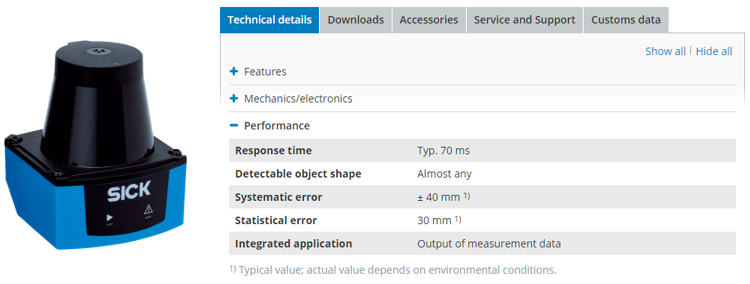
\includegraphics{images/sick-laser.png}
\caption{Example of a possible result}
\end{figure}
Fig. 1: Left, TiM2xx sensor from Sick. Right, performance details of
such sensor.

\(\\[5pt]\)To account for this behavior, sensors' measurements in
probabilistic robotics will be modeled by\ldots{} wait for it\ldots{}
the probability distribution \(p(z|v)\), where z models the measurement
and v is the ground truth.

    \hypertarget{dealing-with-landmark-based-models}{%
\subsection{4.1.1 Dealing with landmark-based
models}\label{dealing-with-landmark-based-models}}

In different applications it is interesting for the robot to detect
landmarks in its workspace and build internal representations of them,
commonly referred to as maps. In the case of maps consisting of a
collection of landmarks \(m=\{m_i\}, i=1,\dots,N\), different types of
sensors can be used to provide observations \(z_i\) of those landmarks:

\begin{itemize}
\tightlist
\item
  \textbf{Distance/range} (\emph{e.g.} radio, GPS, etc.): \(\\[5pt]\)
  \(\hspace{1cm}\) \(z_i = d_i = h_i(x,m)+w_i\) \(\\[5pt]\)
\item
  \textbf{Bearing} (\emph{e.g.} camera): \(\\[5pt]\)
  \(\hspace{1cm}\)\(z_i = \theta_i = h_i(x,m)+w_i\) \(\\[5pt]\)
\item
  \textbf{Distance/range and bearing} (\emph{e.g.} stereo, features in a
  scan, etc.) \(\\[5pt]\)
  \(\hspace{1cm}\)\(z_i = [d_i,\theta_i]^T = h_i(x,m)+w_i\) \emph{(in
  this case, \(h_i(x,m)\) and \(w_i\) are 2D vectors)} \(\\[5pt]\)
\end{itemize}

where:

\begin{itemize}
\tightlist
\item
  \(z_i\) is an observation, \(x\) is the sensor pose, and \(m\) is the
  map of the environment,
\item
  \(h(x,m)\) is the Observation (or measurement, or prediction)
  function: it predicts the value of the observation \(z_i\) given the
  state values \(x\) and \(m\), and
\item
  \(w\) is an error, modeled by a gaussian distribution as
  \(w=[h(x,m)-z_i]\sim N(O,Q)\), being \(Q\) the uncertainty in the
  observation error.
\end{itemize}

In this way, the probability distribution \(p(z|x,m)\) modeling the
sensor measurements results:

\[
p(z|x,m) = K \exp\{-\frac{1}{2}[h(x,m)-z]^T Q^{-1} [h(x,m)-z]\}
\]

These types of maps and sensor measurements pose a new problem:
\textbf{data association}, that is, with which landmark \(m_i\)
correspond the observation \(z_i\) to:

\[h_i(x,m)=h(x,m_i)\]

This problem is usually addressed by applying Chi-squared tests,
although for the shake of simplicity in this book we will consider it as
solved.

    \hypertarget{playing-with-landmarks-and-robot-poses}{%
\subsubsection{Playing with landmarks and robot
poses}\label{playing-with-landmarks-and-robot-poses}}

In the remaining of this section we will familiarize ourselves with the
process of observing landmarks from robots located at certain poses, as
well as the transformations needed to make use of these observations,
that is, to express those observations into the world frame and
backwards.

Some relevant concepts:

\begin{itemize}
\tightlist
\item
  \textbf{World frame}: \((x, y)\) coordinates from a selected point of
  reference \((0, 0)\). We use to keep track of the robots pose, and
  within the map.
\item
  \textbf{Observation}: Information from the real world provided by a
  sensor, from the point of view (\emph{pov}) of a certain robot.
\item
  \textbf{Range-bearing sensor}: Sensor model being used in this lesson.
  This kind of sensors detect how far is an object \((d)\) and its
  orientation relative to the robot's one \((\theta)\).
\end{itemize}

The main tools to deal with those concepts are:

\begin{itemize}
\tightlist
\item
  the composition of two poses.
\item
  the composition of a pose and a landmark.
\item
  the propagation of uncertainty through the Jacobians of these
  compositions.
\end{itemize}

    We will address several problems of incremental complexity. In all of
them, it is important to have in mind how the composition of a (robot)
pose and a landmark point works:

\begin{figure}
\centering
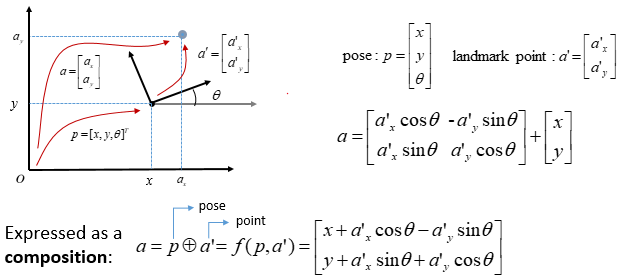
\includegraphics{images/fig4-1.png}
\caption{Example of a possible result}
\end{figure}
Fig. 1: Composition of a pose and a landmark point.

    \begin{tcolorbox}[breakable, size=fbox, boxrule=1pt, pad at break*=1mm,colback=cellbackground, colframe=cellborder]
\prompt{In}{incolor}{1}{\boxspacing}
\begin{Verbatim}[commandchars=\\\{\}]
\PY{c+c1}{\PYZsh{}\PYZpc{}matplotlib notebook}
\PY{o}{\PYZpc{}}\PY{k}{matplotlib} inline

\PY{c+c1}{\PYZsh{} IMPORTS}

\PY{k+kn}{import} \PY{n+nn}{math}
\PY{k+kn}{import} \PY{n+nn}{numpy} \PY{k}{as} \PY{n+nn}{np}
\PY{k+kn}{import} \PY{n+nn}{matplotlib}\PY{n+nn}{.}\PY{n+nn}{pyplot} \PY{k}{as} \PY{n+nn}{plt}
\PY{k+kn}{from} \PY{n+nn}{scipy} \PY{k+kn}{import} \PY{n}{stats}
\PY{k+kn}{from} \PY{n+nn}{numpy} \PY{k+kn}{import} \PY{n}{linalg}

\PY{k+kn}{import} \PY{n+nn}{sys}
\PY{n}{sys}\PY{o}{.}\PY{n}{path}\PY{o}{.}\PY{n}{append}\PY{p}{(}\PY{l+s+s2}{\PYZdq{}}\PY{l+s+s2}{..}\PY{l+s+s2}{\PYZdq{}}\PY{p}{)}
\PY{k+kn}{from} \PY{n+nn}{utils}\PY{n+nn}{.}\PY{n+nn}{PlotEllipse} \PY{k+kn}{import} \PY{n}{PlotEllipse}
\PY{k+kn}{from} \PY{n+nn}{utils}\PY{n+nn}{.}\PY{n+nn}{DrawRobot} \PY{k+kn}{import} \PY{n}{DrawRobot}
\PY{k+kn}{from} \PY{n+nn}{utils}\PY{n+nn}{.}\PY{n+nn}{tcomp} \PY{k+kn}{import} \PY{n}{tcomp}
\PY{k+kn}{from} \PY{n+nn}{utils}\PY{n+nn}{.}\PY{n+nn}{tinv} \PY{k+kn}{import} \PY{n}{tinv}\PY{p}{,} \PY{n}{jac\PYZus{}tinv1} \PY{k}{as} \PY{n}{jac\PYZus{}tinv}
\PY{k+kn}{from} \PY{n+nn}{utils}\PY{n+nn}{.}\PY{n+nn}{Jacobians} \PY{k+kn}{import} \PY{n}{J1}\PY{p}{,} \PY{n}{J2}
\end{Verbatim}
\end{tcolorbox}

    \hypertarget{assignment-1-expressing-an-observed-landmark-in-coordinates-of-the-world-frame}{%
\subsubsection{\texorpdfstring{\textbf{{ASSIGNMENT 1: Expressing an
observed landmark in coordinates of the world frame}}
}{ASSIGNMENT 1: Expressing an observed landmark in coordinates of the world frame }}\label{assignment-1-expressing-an-observed-landmark-in-coordinates-of-the-world-frame}}

Let's consider a robot R1 at a perfectly known pose
\(p_1 = [1, 2, 0.5]^T\) (no uncertainty at this point) which observes a
landmark \(m\) with a range-bearing (polar) sensor affected by a
zero-mean Gaussian error with covariance
\(W_{1p} = diag\left([0.25, 0.04]\right)\). The sensor provides the
measurement \(z_{1p} = [4m., 0.7rad.]^T\). The scenario is the one in
Fig. 2.

\begin{figure}
\centering
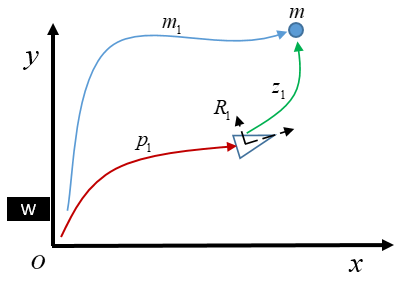
\includegraphics{images/assignment_1.png}
\caption{Example of a possible result}
\end{figure}
Fig 2. Illustration of the scenario in assignment 1.

\textbf{You are tasked to} compute the Gaussian probability distribution
(mean and covariance) of the landmark observation in the world frame
(the same as the robot) and plot its corresponding ellipse (in magenta,
\(\sigma=1\)). Concretely, you have to complete the
\texttt{to\_world\_frame()} function, and modify the demo code to show
the ellipse representing the uncertainty.

Consider the following:

\begin{itemize}
\tightlist
\item
  You can express a sensor measurement in polar coordinates
  (\(z_p=[r,\alpha]^T\)) as cartesian coordinates (\(z_c=[z_x,z_y]^T)\)
  by:
\end{itemize}

\[
     z_c = \begin{bmatrix} z_x \\ z_y \end{bmatrix} 
         = \begin{bmatrix} r \ cos\alpha \\ r \ sin\alpha \end{bmatrix} 
         = f(r,\alpha)
 \] \(\\[5pt]\)

\begin{itemize}
\tightlist
\item
  While computing the covariance of the landmark observation, you have
  to start by computing the covariance of the observation in the
  Cartesian robot \(R1\) frame. That is:
\end{itemize}

\[  
 W_{c} = \frac{\partial f(z_x,z_y)}{\partial \{r,\alpha\}} \ W_{p} \ \frac{\partial f(z_x,z_y)}{\partial \{r,\alpha\}}^T
 \]

Then you can get the convariance in the world frame as:

\[ W_{z\_w} = \frac{\partial f(p,z_c)}{\partial p} \ Q_{p1\_w} \ \left( \frac{\partial f(p,z_c)}{\partial p} \right)^T +
        \frac{\partial f(p,z_c)}{\partial z_c} \ W_{c} \ \left( \frac{\partial f(p,z_c)}{\partial z_c} \right)^T
   \]

where \(f(p,z_c) = p \oplus z_c\), that is, the composition of the pose
and the landmark.

\begin{itemize}
\tightlist
\item
  Note that \(\frac{\partial f(p,z_c)}{\partial p}\) and
  \(\frac{\partial f(p,z_c)}{\partial z_c}\) are the same Jacobians as
  previously used to compose two poses in \emph{robot motion}, but with
  a reduced size since \textbf{while working with landmarks the
  orientation is meaningless, only the position matters}. The functions
  \texttt{J1()} and \texttt{J2()} implement these jacobians for you.
  \(\\[5pt]\)
\end{itemize}

Example: \(\\[5pt]\)

\begin{figure}
\centering
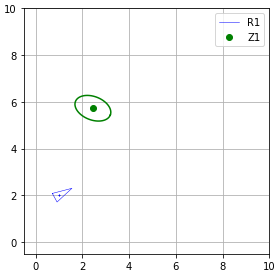
\includegraphics{images/result_1.png}
\caption{Example of a possible result}
\end{figure}
Fig 3. Pose of a robot (without uncertainty) and position of an observed
landmark with its associated uncertainty.

    \begin{tcolorbox}[breakable, size=fbox, boxrule=1pt, pad at break*=1mm,colback=cellbackground, colframe=cellborder]
\prompt{In}{incolor}{2}{\boxspacing}
\begin{Verbatim}[commandchars=\\\{\}]
\PY{k}{def} \PY{n+nf}{to\PYZus{}world\PYZus{}frame}\PY{p}{(}\PY{n}{p1\PYZus{}w}\PY{p}{,} \PY{n}{Qp1\PYZus{}w}\PY{p}{,} \PY{n}{z1\PYZus{}p\PYZus{}r}\PY{p}{,} \PY{n}{W1}\PY{p}{)}\PY{p}{:}
    \PY{l+s+sd}{\PYZdq{}\PYZdq{}\PYZdq{} Covert the observation z1\PYZus{}p\PYZus{}r to the world frame}
\PY{l+s+sd}{    }
\PY{l+s+sd}{        Args:}
\PY{l+s+sd}{            p1\PYZus{}w: Pose of the robot(in world frame)}
\PY{l+s+sd}{            Qp1\PYZus{}w: Covariance of the robot}
\PY{l+s+sd}{            z1\PYZus{}p\PYZus{}r: Observation to a landmark (polar coordinates) from robots perspective}
\PY{l+s+sd}{            W1: Covariance of the sensor in polar coordinates}
\PY{l+s+sd}{    }
\PY{l+s+sd}{        Returns:}
\PY{l+s+sd}{            z1\PYZus{}w: Pose of landmark in the world frame}
\PY{l+s+sd}{            Wz1: Covariance associated to z1\PYZus{}w}
\PY{l+s+sd}{    \PYZdq{}\PYZdq{}\PYZdq{}}
    
    \PY{c+c1}{\PYZsh{} Definition of useful variables}
    \PY{n}{r}\PY{p}{,} \PY{n}{a} \PY{o}{=} \PY{n}{z1\PYZus{}p\PYZus{}r}\PY{p}{[}\PY{l+m+mi}{0}\PY{p}{,}\PY{l+m+mi}{0}\PY{p}{]}\PY{p}{,} \PY{n}{z1\PYZus{}p\PYZus{}r}\PY{p}{[}\PY{l+m+mi}{1}\PY{p}{,}\PY{l+m+mi}{0}\PY{p}{]}
    \PY{n}{s}\PY{p}{,} \PY{n}{c} \PY{o}{=} \PY{n}{np}\PY{o}{.}\PY{n}{sin}\PY{p}{(}\PY{n}{a}\PY{p}{)}\PY{p}{,} \PY{n}{np}\PY{o}{.}\PY{n}{cos}\PY{p}{(}\PY{n}{a}\PY{p}{)}

    \PY{c+c1}{\PYZsh{} Jacobian to convert the measurement uncertainty from polar to cartesian coordinates}
    \PY{n}{Jac\PYZus{}pol\PYZus{}car} \PY{o}{=} \PY{n}{np}\PY{o}{.}\PY{n}{array}\PY{p}{(}\PY{p}{[}
        \PY{p}{[}\PY{n}{c}\PY{p}{,} \PY{o}{\PYZhy{}}\PY{n}{r}\PY{o}{*}\PY{n}{s}\PY{p}{]}\PY{p}{,}
        \PY{p}{[}\PY{n}{s}\PY{p}{,} \PY{n}{r}\PY{o}{*}\PY{n}{c}\PY{p}{]}
    \PY{p}{]}\PY{p}{)}

    \PY{c+c1}{\PYZsh{} Built a tuple with:}
    \PY{c+c1}{\PYZsh{} z1\PYZus{}car\PYZus{}rel[0]: coordinates of the sensor measurement in cartesian coordinates relative to robot position}
    \PY{c+c1}{\PYZsh{} z1\PYZus{}car\PYZus{}rel[1]: its associated uncertainty expressed in cartesian coordinates}
    \PY{n}{z1\PYZus{}car\PYZus{}rel} \PY{o}{=} \PY{p}{(}
            \PY{n}{np}\PY{o}{.}\PY{n}{vstack}\PY{p}{(}\PY{p}{[}\PY{n}{r}\PY{o}{*}\PY{n}{c}\PY{p}{,}\PY{n}{r}\PY{o}{*}\PY{n}{s}\PY{p}{]}\PY{p}{)}\PY{p}{,} \PY{c+c1}{\PYZsh{} position}
            \PY{n}{Jac\PYZus{}pol\PYZus{}car}\PY{n+nd}{@W1}\PY{n+nd}{@Jac\PYZus{}pol\PYZus{}car}\PY{o}{.}\PY{n}{T} \PY{c+c1}{\PYZsh{} uncertainty}
            \PY{p}{)}
    
    \PY{n}{z1\PYZus{}ext} \PY{o}{=} \PY{n}{np}\PY{o}{.}\PY{n}{vstack}\PY{p}{(}\PY{p}{[}\PY{n}{z1\PYZus{}car\PYZus{}rel}\PY{p}{[}\PY{l+m+mi}{0}\PY{p}{]}\PY{p}{,} \PY{l+m+mi}{0}\PY{p}{]}\PY{p}{)} \PY{c+c1}{\PYZsh{} Extends z1 for its usage in the Jacobian functions J1 and J2}

    \PY{c+c1}{\PYZsh{} Build the jacobians }
    \PY{n}{Jac\PYZus{}ap} \PY{o}{=} \PY{n}{J1}\PY{p}{(}\PY{n}{p1\PYZus{}w} \PY{p}{,}\PY{n}{z1\PYZus{}ext}\PY{p}{)}\PY{p}{[}\PY{l+m+mi}{0}\PY{p}{:}\PY{l+m+mi}{2}\PY{p}{,}\PY{p}{:}\PY{p}{]} \PY{c+c1}{\PYZsh{} Jacobian for expressing the uncertainty in the robot pose in a global frame}
    \PY{n}{Jac\PYZus{}aa} \PY{o}{=} \PY{n}{J2}\PY{p}{(}\PY{n}{p1\PYZus{}w} \PY{p}{,}\PY{n}{z1\PYZus{}ext}\PY{p}{)}\PY{p}{[}\PY{l+m+mi}{0}\PY{p}{:}\PY{l+m+mi}{2}\PY{p}{,}\PY{l+m+mi}{0}\PY{p}{:}\PY{l+m+mi}{2}\PY{p}{]} \PY{c+c1}{\PYZsh{} This one expresses the uncertainty in the measurment in a global frame}
    
    \PY{n}{z1\PYZus{}w} \PY{o}{=} \PY{n}{tcomp}\PY{p}{(}\PY{n}{p1\PYZus{}w}\PY{p}{,} \PY{n}{z1\PYZus{}ext}\PY{p}{)}\PY{p}{[}\PY{l+m+mi}{0}\PY{p}{:}\PY{l+m+mi}{2}\PY{p}{,}\PY{p}{[}\PY{l+m+mi}{0}\PY{p}{]}\PY{p}{]} \PY{c+c1}{\PYZsh{} Compute coordinates of the landmark in the world}
    \PY{n}{Wz1} \PY{o}{=} \PY{p}{(}\PY{n}{Jac\PYZus{}ap} \PY{o}{@} \PY{n}{Qp1\PYZus{}w} \PY{o}{@} \PY{n}{Jac\PYZus{}ap}\PY{o}{.}\PY{n}{T}
          \PY{o}{+} \PY{n}{Jac\PYZus{}aa} \PY{o}{@} \PY{n}{z1\PYZus{}car\PYZus{}rel}\PY{p}{[}\PY{l+m+mi}{1}\PY{p}{]} \PY{o}{@} \PY{n}{Jac\PYZus{}aa}\PY{o}{.}\PY{n}{T}\PY{p}{)} \PY{c+c1}{\PYZsh{} Finally, propagate the covariance!}
    
    \PY{k}{return} \PY{n}{z1\PYZus{}w}\PY{p}{,} \PY{n}{Wz1}
\end{Verbatim}
\end{tcolorbox}

    \begin{tcolorbox}[breakable, size=fbox, boxrule=1pt, pad at break*=1mm,colback=cellbackground, colframe=cellborder]
\prompt{In}{incolor}{3}{\boxspacing}
\begin{Verbatim}[commandchars=\\\{\}]
\PY{c+c1}{\PYZsh{} Robot}
\PY{n}{p1\PYZus{}w} \PY{o}{=} \PY{n}{np}\PY{o}{.}\PY{n}{vstack}\PY{p}{(}\PY{p}{[}\PY{l+m+mi}{1}\PY{p}{,} \PY{l+m+mi}{2}\PY{p}{,} \PY{l+m+mf}{0.5}\PY{p}{]}\PY{p}{)} \PY{c+c1}{\PYZsh{} Robot R1 pose}
\PY{n}{Qp1\PYZus{}w} \PY{o}{=} \PY{n}{np}\PY{o}{.}\PY{n}{zeros}\PY{p}{(}\PY{p}{(}\PY{l+m+mi}{3}\PY{p}{,} \PY{l+m+mi}{3}\PY{p}{)}\PY{p}{)} \PY{c+c1}{\PYZsh{} Robot pose convariance matrix (uncertainty)}

\PY{c+c1}{\PYZsh{} Landmark observation}
\PY{n}{z1\PYZus{}p\PYZus{}r} \PY{o}{=} \PY{n}{np}\PY{o}{.}\PY{n}{vstack}\PY{p}{(}\PY{p}{[}\PY{l+m+mf}{4.}\PY{p}{,} \PY{o}{.}\PY{l+m+mi}{7}\PY{p}{]}\PY{p}{)} \PY{c+c1}{\PYZsh{} Measurement/Observation}
\PY{n}{W1} \PY{o}{=} \PY{n}{np}\PY{o}{.}\PY{n}{diag}\PY{p}{(}\PY{p}{[}\PY{l+m+mf}{0.25}\PY{p}{,} \PY{l+m+mf}{0.04}\PY{p}{]}\PY{p}{)} \PY{c+c1}{\PYZsh{} Sensor noise covariance}

\PY{c+c1}{\PYZsh{} Express the landmark observation in the world frame (mean and covariance)}
\PY{n}{z1\PYZus{}w}\PY{p}{,} \PY{n}{Wz1} \PY{o}{=} \PY{n}{to\PYZus{}world\PYZus{}frame}\PY{p}{(}\PY{n}{p1\PYZus{}w}\PY{p}{,} \PY{n}{Qp1\PYZus{}w}\PY{p}{,} \PY{n}{z1\PYZus{}p\PYZus{}r}\PY{p}{,} \PY{n}{W1}\PY{p}{)}

\PY{c+c1}{\PYZsh{} Visualize the results}
\PY{n}{fig}\PY{p}{,} \PY{n}{ax} \PY{o}{=} \PY{n}{plt}\PY{o}{.}\PY{n}{subplots}\PY{p}{(}\PY{p}{)}
\PY{n}{plt}\PY{o}{.}\PY{n}{xlim}\PY{p}{(}\PY{p}{[}\PY{o}{\PYZhy{}}\PY{o}{.}\PY{l+m+mi}{5}\PY{p}{,} \PY{l+m+mi}{10}\PY{p}{]}\PY{p}{)}
\PY{n}{plt}\PY{o}{.}\PY{n}{ylim}\PY{p}{(}\PY{p}{[}\PY{o}{\PYZhy{}}\PY{o}{.}\PY{l+m+mi}{5}\PY{p}{,} \PY{l+m+mi}{10}\PY{p}{]}\PY{p}{)}
\PY{n}{plt}\PY{o}{.}\PY{n}{grid}\PY{p}{(}\PY{p}{)}
\PY{n}{plt}\PY{o}{.}\PY{n}{tight\PYZus{}layout}\PY{p}{(}\PY{p}{)}

\PY{n}{DrawRobot}\PY{p}{(}\PY{n}{fig}\PY{p}{,} \PY{n}{ax}\PY{p}{,} \PY{n}{p1\PYZus{}w}\PY{p}{,} \PY{n}{label}\PY{o}{=}\PY{l+s+s1}{\PYZsq{}}\PY{l+s+s1}{R1}\PY{l+s+s1}{\PYZsq{}}\PY{p}{,} \PY{n}{color}\PY{o}{=}\PY{l+s+s1}{\PYZsq{}}\PY{l+s+s1}{blue}\PY{l+s+s1}{\PYZsq{}}\PY{p}{)}
    
\PY{n}{ax}\PY{o}{.}\PY{n}{plot}\PY{p}{(}\PY{n}{z1\PYZus{}w}\PY{p}{[}\PY{l+m+mi}{0}\PY{p}{,} \PY{l+m+mi}{0}\PY{p}{]}\PY{p}{,} \PY{n}{z1\PYZus{}w}\PY{p}{[}\PY{l+m+mi}{1}\PY{p}{,} \PY{l+m+mi}{0}\PY{p}{]}\PY{p}{,} \PY{l+s+s1}{\PYZsq{}}\PY{l+s+s1}{o}\PY{l+s+s1}{\PYZsq{}}\PY{p}{,} \PY{n}{label}\PY{o}{=}\PY{l+s+s1}{\PYZsq{}}\PY{l+s+s1}{Z1}\PY{l+s+s1}{\PYZsq{}}\PY{p}{,} \PY{n}{color}\PY{o}{=}\PY{l+s+s1}{\PYZsq{}}\PY{l+s+s1}{green}\PY{l+s+s1}{\PYZsq{}}\PY{p}{)}
\PY{n}{PlotEllipse}\PY{p}{(}\PY{n}{fig}\PY{p}{,} \PY{n}{ax}\PY{p}{,} \PY{n}{z1\PYZus{}w}\PY{p}{,} \PY{n}{Wz1}\PY{p}{,} \PY{n}{color}\PY{o}{=}\PY{l+s+s1}{\PYZsq{}}\PY{l+s+s1}{green}\PY{l+s+s1}{\PYZsq{}}\PY{p}{)}

\PY{n}{plt}\PY{o}{.}\PY{n}{legend}\PY{p}{(}\PY{p}{)}
\PY{n+nb}{print}\PY{p}{(}\PY{l+s+s1}{\PYZsq{}}\PY{l+s+s1}{\PYZhy{}\PYZhy{}\PYZhy{}\PYZhy{}}\PY{l+s+se}{\PYZbs{}t}\PY{l+s+s1}{Exercise 4.1.1}\PY{l+s+se}{\PYZbs{}t}\PY{l+s+s1}{\PYZhy{}\PYZhy{}\PYZhy{}\PYZhy{}}\PY{l+s+se}{\PYZbs{}n}\PY{l+s+s1}{\PYZsq{}}\PY{o}{+}
      \PY{l+s+s1}{\PYZsq{}}\PY{l+s+s1}{z1\PYZus{}w = }\PY{l+s+si}{\PYZob{}\PYZcb{}}\PY{l+s+se}{\PYZbs{}\PYZsq{}}\PY{l+s+se}{\PYZbs{}n}\PY{l+s+s1}{\PYZsq{}}\PY{o}{.}\PY{n}{format}\PY{p}{(}\PY{n}{z1\PYZus{}w}\PY{o}{.}\PY{n}{flatten}\PY{p}{(}\PY{p}{)}\PY{p}{)}
      \PY{o}{+} \PY{l+s+s1}{\PYZsq{}}\PY{l+s+s1}{Wz1\PYZus{}w = }\PY{l+s+se}{\PYZbs{}n}\PY{l+s+si}{\PYZob{}\PYZcb{}}\PY{l+s+se}{\PYZbs{}n}\PY{l+s+s1}{\PYZsq{}}\PY{o}{.}\PY{n}{format}\PY{p}{(}\PY{n}{Wz1}\PY{p}{)}\PY{p}{)}
\end{Verbatim}
\end{tcolorbox}

    \begin{Verbatim}[commandchars=\\\{\}]
----    Exercise 4.1.1  ----
z1\_w = [2.44943102 5.72815634]'
Wz1\_w =
[[ 0.58879177 -0.13171532]
 [-0.13171532  0.30120823]]

    \end{Verbatim}

    \begin{center}
    \adjustimage{max size={0.9\linewidth}{0.9\paperheight}}{output_8_1.png}
    \end{center}
    { \hspace*{\fill} \\}
    
    {Expected results for demo:}

\begin{verbatim}
---- Exercise 4.1.1 ----
z1_w = [2.44943102 5.72815634]'
Wz1_w = 
[[ 0.58879177 -0.13171532]
 [-0.13171532  0.30120823]]
\end{verbatim}

    \hypertarget{assignment-2-adding-uncertainty-to-the-robot-position}{%
\subsubsection{\texorpdfstring{\textbf{{ASSIGNMENT 2: Adding uncertainty
to the robot
position}}}{ASSIGNMENT 2: Adding uncertainty to the robot position}}\label{assignment-2-adding-uncertainty-to-the-robot-position}}

Now, let's assume that the robot pose is not known, but it is a RV that
follows a Gaussian probability distribution:
\(p_1 \sim N([1, 2, 0.5]^T, \Sigma_1)\) with
\(\Sigma_1 = diag([0.08,0.6, 0.02 ])\).

\begin{enumerate}
\def\labelenumi{\arabic{enumi}.}
\item
  Compute the covariance matrix \(\Sigma_{m1}\) of the landmark in the
  world frame and plot it as an ellipse centered at the mean \(m_1\) (in
  blue, \(sigma= 1\)). Plot also the covariance of the robot pose (in
  blue, \(sigma= 1\)).
\item
  Compare the covariance with that obtained in the previous case.
  \(\\[5pt]\)
\end{enumerate}

Example: \(\\[5pt]\)
\begin{figure}
\centering
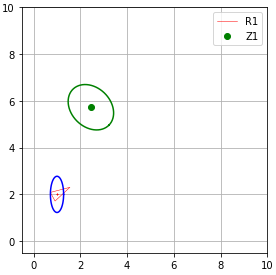
\includegraphics{images/result_2.png}
\caption{Example of a possible result}
\end{figure}
Fig 4. Pose of a robot and position of an observed landmark, along with
their associated uncertainties.

    \begin{tcolorbox}[breakable, size=fbox, boxrule=1pt, pad at break*=1mm,colback=cellbackground, colframe=cellborder]
\prompt{In}{incolor}{4}{\boxspacing}
\begin{Verbatim}[commandchars=\\\{\}]
\PY{c+c1}{\PYZsh{} Robot}
\PY{n}{p1\PYZus{}w} \PY{o}{=} \PY{n}{np}\PY{o}{.}\PY{n}{vstack}\PY{p}{(}\PY{p}{[}\PY{l+m+mi}{1}\PY{p}{,} \PY{l+m+mi}{2}\PY{p}{,} \PY{l+m+mf}{0.5}\PY{p}{]}\PY{p}{)} \PY{c+c1}{\PYZsh{} Robot R1 pose}
\PY{n}{Qp1\PYZus{}w} \PY{o}{=} \PY{n}{np}\PY{o}{.}\PY{n}{diag}\PY{p}{(}\PY{p}{[}\PY{l+m+mf}{0.08}\PY{p}{,}\PY{l+m+mf}{0.6}\PY{p}{,}\PY{l+m+mf}{0.02}\PY{p}{]}\PY{p}{)}  \PY{c+c1}{\PYZsh{} Robot pose convariance matrix (uncertainty)}

\PY{c+c1}{\PYZsh{} Landmark observation}
\PY{n}{z1\PYZus{}p\PYZus{}r} \PY{o}{=} \PY{n}{np}\PY{o}{.}\PY{n}{vstack}\PY{p}{(}\PY{p}{[}\PY{l+m+mf}{4.}\PY{p}{,} \PY{o}{.}\PY{l+m+mi}{7}\PY{p}{]}\PY{p}{)} \PY{c+c1}{\PYZsh{} Measurement/Observation}
\PY{n}{W1} \PY{o}{=} \PY{n}{np}\PY{o}{.}\PY{n}{diag}\PY{p}{(}\PY{p}{[}\PY{l+m+mf}{0.25}\PY{p}{,} \PY{l+m+mf}{0.04}\PY{p}{]}\PY{p}{)} \PY{c+c1}{\PYZsh{} Sensor noise covariance}

\PY{c+c1}{\PYZsh{} Express the landmark observation in the world frame (mean and covariance)}
\PY{n}{z1\PYZus{}w}\PY{p}{,} \PY{n}{Wz1} \PY{o}{=} \PY{n}{to\PYZus{}world\PYZus{}frame}\PY{p}{(}\PY{n}{p1\PYZus{}w}\PY{p}{,} \PY{n}{Qp1\PYZus{}w}\PY{p}{,} \PY{n}{z1\PYZus{}p\PYZus{}r}\PY{p}{,} \PY{n}{W1}\PY{p}{)}

\PY{c+c1}{\PYZsh{} MATPLOTLIB}
\PY{n}{fig}\PY{p}{,} \PY{n}{ax} \PY{o}{=} \PY{n}{plt}\PY{o}{.}\PY{n}{subplots}\PY{p}{(}\PY{p}{)}
\PY{n}{plt}\PY{o}{.}\PY{n}{xlim}\PY{p}{(}\PY{p}{[}\PY{o}{\PYZhy{}}\PY{o}{.}\PY{l+m+mi}{5}\PY{p}{,} \PY{l+m+mi}{10}\PY{p}{]}\PY{p}{)}
\PY{n}{plt}\PY{o}{.}\PY{n}{ylim}\PY{p}{(}\PY{p}{[}\PY{o}{\PYZhy{}}\PY{o}{.}\PY{l+m+mi}{5}\PY{p}{,} \PY{l+m+mi}{10}\PY{p}{]}\PY{p}{)}
\PY{n}{plt}\PY{o}{.}\PY{n}{grid}\PY{p}{(}\PY{p}{)}
\PY{n}{plt}\PY{o}{.}\PY{n}{tight\PYZus{}layout}\PY{p}{(}\PY{p}{)}

\PY{n}{fig}\PY{o}{.}\PY{n}{canvas}\PY{o}{.}\PY{n}{draw}\PY{p}{(}\PY{p}{)}

\PY{n}{DrawRobot}\PY{p}{(}\PY{n}{fig}\PY{p}{,} \PY{n}{ax}\PY{p}{,} \PY{n}{p1\PYZus{}w}\PY{p}{,} \PY{n}{label}\PY{o}{=}\PY{l+s+s1}{\PYZsq{}}\PY{l+s+s1}{R1}\PY{l+s+s1}{\PYZsq{}}\PY{p}{,} \PY{n}{color}\PY{o}{=}\PY{l+s+s1}{\PYZsq{}}\PY{l+s+s1}{red}\PY{l+s+s1}{\PYZsq{}}\PY{p}{)}  
\PY{n}{PlotEllipse}\PY{p}{(}\PY{n}{fig}\PY{p}{,} \PY{n}{ax}\PY{p}{,} \PY{n}{p1\PYZus{}w}\PY{p}{,} \PY{n}{Qp1\PYZus{}w}\PY{p}{,} \PY{n}{color}\PY{o}{=}\PY{l+s+s1}{\PYZsq{}}\PY{l+s+s1}{blue}\PY{l+s+s1}{\PYZsq{}}\PY{p}{)}

\PY{n}{ax}\PY{o}{.}\PY{n}{plot}\PY{p}{(}\PY{n}{z1\PYZus{}w}\PY{p}{[}\PY{l+m+mi}{0}\PY{p}{,} \PY{l+m+mi}{0}\PY{p}{]}\PY{p}{,} \PY{n}{z1\PYZus{}w}\PY{p}{[}\PY{l+m+mi}{1}\PY{p}{,} \PY{l+m+mi}{0}\PY{p}{]}\PY{p}{,} \PY{l+s+s1}{\PYZsq{}}\PY{l+s+s1}{o}\PY{l+s+s1}{\PYZsq{}}\PY{p}{,} \PY{n}{label}\PY{o}{=}\PY{l+s+s1}{\PYZsq{}}\PY{l+s+s1}{Z1}\PY{l+s+s1}{\PYZsq{}}\PY{p}{,} \PY{n}{color}\PY{o}{=}\PY{l+s+s1}{\PYZsq{}}\PY{l+s+s1}{green}\PY{l+s+s1}{\PYZsq{}}\PY{p}{)}
\PY{n}{PlotEllipse}\PY{p}{(}\PY{n}{fig}\PY{p}{,} \PY{n}{ax}\PY{p}{,} \PY{n}{z1\PYZus{}w}\PY{p}{,} \PY{n}{Wz1}\PY{p}{,} \PY{n}{color}\PY{o}{=}\PY{l+s+s1}{\PYZsq{}}\PY{l+s+s1}{green}\PY{l+s+s1}{\PYZsq{}}\PY{p}{)}

\PY{n}{plt}\PY{o}{.}\PY{n}{legend}\PY{p}{(}\PY{p}{)}
\PY{n+nb}{print}\PY{p}{(}\PY{l+s+s1}{\PYZsq{}}\PY{l+s+s1}{\PYZhy{}\PYZhy{}\PYZhy{}\PYZhy{} Exercise 4.1.2 \PYZhy{}\PYZhy{}\PYZhy{}\PYZhy{}}\PY{l+s+se}{\PYZbs{}n}\PY{l+s+s1}{\PYZsq{}}\PY{o}{+}
      \PY{l+s+s1}{\PYZsq{}}\PY{l+s+s1}{Wz1\PYZus{}w = }\PY{l+s+se}{\PYZbs{}n}\PY{l+s+si}{\PYZob{}\PYZcb{}}\PY{l+s+se}{\PYZbs{}n}\PY{l+s+s1}{\PYZsq{}}\PY{o}{.}\PY{n}{format}\PY{p}{(}\PY{n}{Wz1}\PY{p}{)}\PY{p}{)}
\end{Verbatim}
\end{tcolorbox}

    \begin{Verbatim}[commandchars=\\\{\}]
---- Exercise 4.1.2 ----
Wz1\_w =
[[ 0.94677477 -0.23978943]
 [-0.23978943  0.94322523]]

    \end{Verbatim}

    \begin{center}
    \adjustimage{max size={0.9\linewidth}{0.9\paperheight}}{output_11_1.png}
    \end{center}
    { \hspace*{\fill} \\}
    
    {Expected results for demo:}

\begin{verbatim}
---- Exercise 4.1.2 ----
Wz1_w = 
[[ 0.94677477 -0.23978943]
 [-0.23978943  0.94322523]]
\end{verbatim}

    \hypertarget{assignment-3-getting-the-relative-pose-between-two-robots}{%
\subsubsection{\texorpdfstring{\textbf{{ASSIGNMENT 3: Getting the
relative pose between two
robots}}}{ASSIGNMENT 3: Getting the relative pose between two robots}}\label{assignment-3-getting-the-relative-pose-between-two-robots}}

Another robot \texttt{R2} is at pose
\(p_2 \sim ([6m., 4m., 2.1rad.]^T, \Sigma_2)\) with
\(\Sigma_2 = diag([0.20,0.09,  0.03])\). Plot \texttt{p2} and its
ellipse (covariance) in green (\(sigma=1\)). \textbf{Compute the
relative pose \texttt{p12} between \texttt{R1} and \texttt{R2}},
including its associated uncertainty. This scenario is shown in Fig. 5.

\begin{figure}
\centering
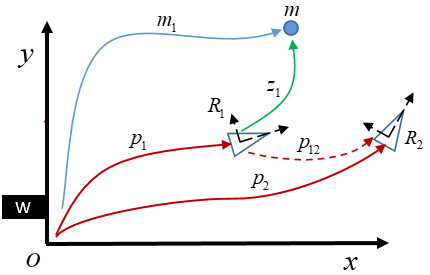
\includegraphics{images/assignment_3.png}
\caption{Example of a possible result}
\end{figure}
Fig 5. Illustration of the scenario in this assignment.

This relative pose can be obtained in two different ways: -
\textbf{Through the composition of poses}, but using \(\ominus p1\)
instead of \(p1\). Implement it in \texttt{inverse\_composition1()}.

Mean:

\[
 p12 = \ominus p1 \oplus p2 = f(\ominus p1, p2) = 
 \begin{bmatrix} 
  x_{\ominus p1} + x_{p2} cos \theta_{\ominus p1} - y_{p2} sin \theta_{\ominus p1} \\
  y_{\ominus p1} + x_{p2} sin \theta_{\ominus p1} + y_{p2} cos \theta_{\ominus p1} \\
  \theta_{\ominus p1} + \theta_{p2}
 \end{bmatrix}
 \]

Covariance:

\[
 \Sigma_{p12} = \frac{\partial p12}{\partial \ominus p1} \frac{\ominus p1}{\partial p1} \Sigma_{p1} \frac{\ominus p1}{\partial p1}^T \frac{\partial p12}{\partial \ominus p1}^T 
 +
 \frac{\partial p12}{\partial p2} \Sigma_{p2}  \frac{\partial p12}{\partial p2}^T
 \\
 \text{Applying the Chain rule} \rightarrow \Sigma_{p12} = \frac{\partial p12}{\partial \ominus p1} \Sigma_{\ominus p1} \frac{\partial p12}{\partial \ominus p1}^T
 +
 \frac{\partial p12}{\partial p2} \Sigma_{p2}  \frac{\partial p12}{\partial p2}^T
 \]

Being:

\[
 \frac{\partial p12}{\partial \ominus p1} = 
 \begin{bmatrix}
 1 & 0 & -x_{p2} sin \theta_{\ominus p1} - y_{p2} cos \theta_{\ominus p1} \\
 0 & 1 & x_{p2} cos \theta_{\ominus p1} - y_{p2} sin \theta_{\ominus p1} \\
 0 & 0 & 1
 \end{bmatrix}  
 \; \; \; \; \; \frac{\partial p12}{\partial p2} = 
 \begin{bmatrix}
cos \theta_{\ominus p1} & -sin \theta_{\ominus p1} & 0\\
sin \theta_{\ominus p1} & cos \theta_{\ominus p1} & 0\\
 0 & 0 & 1
 \end{bmatrix}
\] \(\\[5pt]\)

\[
 \frac{\partial \ominus p1}{\partial p1} = 
 \begin{bmatrix}
 -cos \theta_{p1} & -sin \theta_{p1} & x_{p1} sin \theta_{p1} - y_{p1} cos \theta_{p1} \\
 sin \theta_{p1} & -cos \theta_{p1} & x_{p1} cos \theta_{p1} + y_{p1} sin \theta_{p1}\\
 0 & 0 & -1 \\
 \end{bmatrix}
 \; \; \; \; \; \Sigma_{\ominus p1} = \frac{\partial \ominus p1}{\partial p1} \Sigma_{p1} \frac{\partial \ominus p1}{\partial p1}^T
 \] \(\\[5pt]\)

\begin{itemize}
\tightlist
\item
  \textbf{Using the inverse composition of poses}. This one is given for
  you in \texttt{inverse\_composition2()}.
\end{itemize}

    \begin{tcolorbox}[breakable, size=fbox, boxrule=1pt, pad at break*=1mm,colback=cellbackground, colframe=cellborder]
\prompt{In}{incolor}{5}{\boxspacing}
\begin{Verbatim}[commandchars=\\\{\}]
\PY{k}{def} \PY{n+nf}{inverse\PYZus{}composition1}\PY{p}{(}\PY{n}{p1\PYZus{}w}\PY{p}{,} \PY{n}{Qp1\PYZus{}w}\PY{p}{,} \PY{n}{p2\PYZus{}w}\PY{p}{,} \PY{n}{Qp2\PYZus{}w}\PY{p}{)}\PY{p}{:}
    \PY{n}{jac\PYZus{}inv\PYZus{}p} \PY{o}{=} \PY{n}{jac\PYZus{}tinv}\PY{p}{(}\PY{n}{p1\PYZus{}w}\PY{p}{)}

    \PY{n}{inv\PYZus{}r1} \PY{o}{=} \PY{p}{(}
        \PY{n}{tinv}\PY{p}{(}\PY{n}{p1\PYZus{}w}\PY{p}{)}\PY{p}{,}
        \PY{n}{jac\PYZus{}inv\PYZus{}p} \PY{o}{@} \PY{n}{Qp1\PYZus{}w} \PY{o}{@} \PY{n}{jac\PYZus{}inv\PYZus{}p}\PY{o}{.}\PY{n}{T}
    \PY{p}{)}

    \PY{n}{jac\PYZus{}p12\PYZus{}inv} \PY{o}{=} \PY{n}{J1}\PY{p}{(}\PY{n}{inv\PYZus{}r1}\PY{p}{[}\PY{l+m+mi}{0}\PY{p}{]}\PY{p}{,} \PY{n}{p2\PYZus{}w}\PY{p}{)}
    \PY{n}{jac\PYZus{}p12\PYZus{}p2} \PY{o}{=} \PY{n}{J2}\PY{p}{(}\PY{n}{inv\PYZus{}r1}\PY{p}{[}\PY{l+m+mi}{0}\PY{p}{]}\PY{p}{,} \PY{n}{p2\PYZus{}w}\PY{p}{)}

    \PY{n}{p12\PYZus{}w} \PY{o}{=} \PY{n}{tcomp}\PY{p}{(}\PY{n}{inv\PYZus{}r1}\PY{p}{[}\PY{l+m+mi}{0}\PY{p}{]}\PY{p}{,} \PY{n}{p2\PYZus{}w}\PY{p}{)}
    
    \PY{n}{Qp12\PYZus{}w} \PY{o}{=} \PY{p}{(}
            \PY{n}{jac\PYZus{}p12\PYZus{}inv}\PY{n+nd}{@inv\PYZus{}r1}\PY{p}{[}\PY{l+m+mi}{1}\PY{p}{]}\PY{n+nd}{@jac\PYZus{}p12\PYZus{}inv}\PY{o}{.}\PY{n}{T} 
            \PY{o}{+} \PY{n}{jac\PYZus{}p12\PYZus{}p2}\PY{n+nd}{@Qp2\PYZus{}w}\PY{n+nd}{@jac\PYZus{}p12\PYZus{}p2}\PY{o}{.}\PY{n}{T}
        \PY{p}{)}
    
    \PY{k}{return} \PY{n}{p12\PYZus{}w}\PY{p}{,} \PY{n}{Qp12\PYZus{}w}
\end{Verbatim}
\end{tcolorbox}

    \begin{tcolorbox}[breakable, size=fbox, boxrule=1pt, pad at break*=1mm,colback=cellbackground, colframe=cellborder]
\prompt{In}{incolor}{6}{\boxspacing}
\begin{Verbatim}[commandchars=\\\{\}]
\PY{k}{def} \PY{n+nf}{inverse\PYZus{}composition2}\PY{p}{(}\PY{n}{p1\PYZus{}w}\PY{p}{,} \PY{n}{Qp1\PYZus{}w}\PY{p}{,} \PY{n}{p2\PYZus{}w}\PY{p}{,} \PY{n}{Qp2\PYZus{}w}\PY{p}{)}\PY{p}{:}
    \PY{n}{dx}\PY{p}{,} \PY{n}{dy} \PY{o}{=} \PY{n}{p2\PYZus{}w}\PY{p}{[}\PY{l+m+mi}{0}\PY{p}{,} \PY{l+m+mi}{0}\PY{p}{]}\PY{o}{\PYZhy{}}\PY{n}{p1\PYZus{}w}\PY{p}{[}\PY{l+m+mi}{0}\PY{p}{,} \PY{l+m+mi}{0}\PY{p}{]}\PY{p}{,} \PY{n}{p2\PYZus{}w}\PY{p}{[}\PY{l+m+mi}{1}\PY{p}{,} \PY{l+m+mi}{0}\PY{p}{]}\PY{o}{\PYZhy{}}\PY{n}{p1\PYZus{}w}\PY{p}{[}\PY{l+m+mi}{1}\PY{p}{,} \PY{l+m+mi}{0}\PY{p}{]}
    \PY{n}{a} \PY{o}{=} \PY{n}{p2\PYZus{}w}\PY{p}{[}\PY{l+m+mi}{2}\PY{p}{,} \PY{l+m+mi}{0}\PY{p}{]} \PY{o}{\PYZhy{}} \PY{n}{p1\PYZus{}w}\PY{p}{[}\PY{l+m+mi}{2}\PY{p}{,} \PY{l+m+mi}{0}\PY{p}{]}
    \PY{n}{c}\PY{p}{,} \PY{n}{s} \PY{o}{=} \PY{n}{np}\PY{o}{.}\PY{n}{cos}\PY{p}{(}\PY{n}{p1\PYZus{}w}\PY{p}{[}\PY{l+m+mi}{2}\PY{p}{,} \PY{l+m+mi}{0}\PY{p}{]}\PY{p}{)}\PY{p}{,} \PY{n}{np}\PY{o}{.}\PY{n}{sin}\PY{p}{(}\PY{n}{p1\PYZus{}w}\PY{p}{[}\PY{l+m+mi}{2}\PY{p}{,} \PY{l+m+mi}{0}\PY{p}{]}\PY{p}{)}

    \PY{n}{p12\PYZus{}w} \PY{o}{=} \PY{n}{np}\PY{o}{.}\PY{n}{array}\PY{p}{(}\PY{p}{[}
        \PY{p}{[}\PY{n}{dx}\PY{o}{*}\PY{n}{c} \PY{o}{+} \PY{n}{dy}\PY{o}{*}\PY{n}{s}\PY{p}{]}\PY{p}{,}
        \PY{p}{[}\PY{o}{\PYZhy{}}\PY{n}{dx}\PY{o}{*}\PY{n}{s} \PY{o}{+} \PY{n}{dy}\PY{o}{*}\PY{n}{c}\PY{p}{]}\PY{p}{,}
        \PY{p}{[}\PY{n}{a}\PY{p}{]}\PY{p}{]}\PY{p}{)}
    
    
    \PY{n}{jac\PYZus{}p12\PYZus{}r1} \PY{o}{=} \PY{n}{np}\PY{o}{.}\PY{n}{array}\PY{p}{(}\PY{p}{[}
        \PY{p}{[}\PY{o}{\PYZhy{}}\PY{n}{c}\PY{p}{,} \PY{o}{\PYZhy{}}\PY{n}{s}\PY{p}{,} \PY{o}{\PYZhy{}}\PY{n}{dx}\PY{o}{*}\PY{n}{s} \PY{o}{+} \PY{n}{dy}\PY{o}{*}\PY{n}{c}\PY{p}{]}\PY{p}{,}
        \PY{p}{[}\PY{n}{s}\PY{p}{,} \PY{o}{\PYZhy{}}\PY{n}{c}\PY{p}{,} \PY{o}{\PYZhy{}}\PY{n}{dx}\PY{o}{*}\PY{n}{c} \PY{o}{\PYZhy{}} \PY{n}{dy}\PY{o}{*}\PY{n}{s}\PY{p}{]}\PY{p}{,}
        \PY{p}{[}\PY{l+m+mi}{0}\PY{p}{,} \PY{l+m+mi}{0}\PY{p}{,} \PY{o}{\PYZhy{}}\PY{l+m+mi}{1}\PY{p}{]}
    \PY{p}{]}\PY{p}{)}

    \PY{n}{jac\PYZus{}p12\PYZus{}r2} \PY{o}{=} \PY{n}{np}\PY{o}{.}\PY{n}{array}\PY{p}{(}\PY{p}{[}
        \PY{p}{[}\PY{n}{c}\PY{p}{,} \PY{n}{s}\PY{p}{,} \PY{l+m+mi}{0}\PY{p}{]}\PY{p}{,}
        \PY{p}{[}\PY{o}{\PYZhy{}}\PY{n}{s}\PY{p}{,} \PY{n}{c}\PY{p}{,} \PY{l+m+mi}{0}\PY{p}{]}\PY{p}{,}
        \PY{p}{[}\PY{l+m+mi}{0}\PY{p}{,} \PY{l+m+mi}{0}\PY{p}{,} \PY{o}{\PYZhy{}}\PY{l+m+mi}{1}\PY{p}{]}
    \PY{p}{]}\PY{p}{)}

    \PY{c+c1}{\PYZsh{}jac\PYZus{}p1\PYZus{}pinv = np.linalg.inv(jac\PYZus{}tinv(r1[0]))}

    \PY{n}{Qp12\PYZus{}w} \PY{o}{=} \PY{n}{jac\PYZus{}p12\PYZus{}r1}\PY{n+nd}{@Qp1\PYZus{}w}\PY{n+nd}{@jac\PYZus{}p12\PYZus{}r1}\PY{o}{.}\PY{n}{T} \PY{o}{+} \PY{n}{jac\PYZus{}p12\PYZus{}r2}\PY{n+nd}{@Qp2\PYZus{}w}\PY{n+nd}{@jac\PYZus{}p12\PYZus{}r2}\PY{o}{.}\PY{n}{T}

    \PY{k}{return} \PY{n}{p12\PYZus{}w}\PY{p}{,} \PY{n}{Qp12\PYZus{}w}
\end{Verbatim}
\end{tcolorbox}

    \begin{tcolorbox}[breakable, size=fbox, boxrule=1pt, pad at break*=1mm,colback=cellbackground, colframe=cellborder]
\prompt{In}{incolor}{7}{\boxspacing}
\begin{Verbatim}[commandchars=\\\{\}]
\PY{c+c1}{\PYZsh{} Robot R1}
\PY{n}{p1\PYZus{}w} \PY{o}{=} \PY{n}{np}\PY{o}{.}\PY{n}{vstack}\PY{p}{(}\PY{p}{[}\PY{l+m+mf}{1.}\PY{p}{,} \PY{l+m+mf}{2.}\PY{p}{,} \PY{l+m+mf}{0.5}\PY{p}{]}\PY{p}{)}
\PY{n}{Qp1\PYZus{}w} \PY{o}{=} \PY{n}{np}\PY{o}{.}\PY{n}{diag}\PY{p}{(}\PY{p}{[}\PY{l+m+mf}{0.08}\PY{p}{,} \PY{l+m+mf}{0.6}\PY{p}{,} \PY{l+m+mf}{0.02}\PY{p}{]}\PY{p}{)}

\PY{c+c1}{\PYZsh{} Robot R2}
\PY{n}{p2\PYZus{}w} \PY{o}{=} \PY{n}{np}\PY{o}{.}\PY{n}{vstack}\PY{p}{(}\PY{p}{[}\PY{l+m+mf}{6.}\PY{p}{,} \PY{l+m+mf}{4.}\PY{p}{,} \PY{l+m+mf}{2.1}\PY{p}{]}\PY{p}{)}
\PY{n}{Qp2\PYZus{}w} \PY{o}{=} \PY{n}{np}\PY{o}{.}\PY{n}{diag}\PY{p}{(}\PY{p}{[}\PY{l+m+mf}{0.20}\PY{p}{,} \PY{l+m+mf}{0.09}\PY{p}{,} \PY{l+m+mf}{0.03}\PY{p}{]}\PY{p}{)}

\PY{c+c1}{\PYZsh{} Obtain the relative pose p12 between both robots through the composition of poses}
\PY{n}{p12\PYZus{}w}\PY{p}{,} \PY{n}{Qp12\PYZus{}w} \PY{o}{=} \PY{n}{inverse\PYZus{}composition1}\PY{p}{(}\PY{n}{p1\PYZus{}w}\PY{p}{,} \PY{n}{Qp1\PYZus{}w}\PY{p}{,} \PY{n}{p2\PYZus{}w}\PY{p}{,} \PY{n}{Qp2\PYZus{}w}\PY{p}{)}
\PY{n+nb}{print}\PY{p}{(} \PY{l+s+s1}{\PYZsq{}}\PY{l+s+s1}{\PYZhy{}\PYZhy{}\PYZhy{}\PYZhy{}}\PY{l+s+se}{\PYZbs{}t}\PY{l+s+s1}{Exercise 4.1.3 with method 1}\PY{l+s+se}{\PYZbs{}t}\PY{l+s+s1}{\PYZhy{}\PYZhy{}\PYZhy{}\PYZhy{}}\PY{l+s+se}{\PYZbs{}n}\PY{l+s+s1}{\PYZsq{}}\PY{o}{+}
        \PY{l+s+s1}{\PYZsq{}}\PY{l+s+s1}{p12\PYZus{}w = }\PY{l+s+si}{\PYZob{}\PYZcb{}}\PY{l+s+se}{\PYZbs{}\PYZsq{}}\PY{l+s+se}{\PYZbs{}n}\PY{l+s+s1}{\PYZsq{}}\PY{o}{.}\PY{n}{format}\PY{p}{(}\PY{n}{p12\PYZus{}w}\PY{o}{.}\PY{n}{flatten}\PY{p}{(}\PY{p}{)}\PY{p}{)}\PY{o}{+}
        \PY{l+s+s1}{\PYZsq{}}\PY{l+s+s1}{Qp12\PYZus{}w = }\PY{l+s+se}{\PYZbs{}n}\PY{l+s+si}{\PYZob{}\PYZcb{}}\PY{l+s+se}{\PYZbs{}n}\PY{l+s+s1}{\PYZsq{}}\PY{o}{.}\PY{n}{format}\PY{p}{(}\PY{n}{Qp12\PYZus{}w}\PY{p}{)}\PY{p}{)}

\PY{c+c1}{\PYZsh{} Obtain the relative pose p12 between both robots through the inverse composition of poses}
\PY{n}{p12\PYZus{}w}\PY{p}{,} \PY{n}{Qp12\PYZus{}w} \PY{o}{=} \PY{n}{inverse\PYZus{}composition2}\PY{p}{(}\PY{n}{p1\PYZus{}w}\PY{p}{,} \PY{n}{Qp1\PYZus{}w}\PY{p}{,} \PY{n}{p2\PYZus{}w}\PY{p}{,} \PY{n}{Qp2\PYZus{}w}\PY{p}{)}
\PY{n+nb}{print}\PY{p}{(} \PY{l+s+s1}{\PYZsq{}}\PY{l+s+s1}{\PYZhy{}\PYZhy{}\PYZhy{}\PYZhy{}}\PY{l+s+se}{\PYZbs{}t}\PY{l+s+s1}{Exercise 4.1.3 with method 2}\PY{l+s+se}{\PYZbs{}t}\PY{l+s+s1}{\PYZhy{}\PYZhy{}\PYZhy{}\PYZhy{}}\PY{l+s+se}{\PYZbs{}n}\PY{l+s+s1}{\PYZsq{}}\PY{o}{+}
        \PY{l+s+s1}{\PYZsq{}}\PY{l+s+s1}{p12\PYZus{}w = }\PY{l+s+si}{\PYZob{}\PYZcb{}}\PY{l+s+se}{\PYZbs{}\PYZsq{}}\PY{l+s+se}{\PYZbs{}n}\PY{l+s+s1}{\PYZsq{}}\PY{o}{.}\PY{n}{format}\PY{p}{(}\PY{n}{p12\PYZus{}w}\PY{o}{.}\PY{n}{flatten}\PY{p}{(}\PY{p}{)}\PY{p}{)}\PY{o}{+}
        \PY{l+s+s1}{\PYZsq{}}\PY{l+s+s1}{Qp12\PYZus{}w = }\PY{l+s+se}{\PYZbs{}n}\PY{l+s+si}{\PYZob{}\PYZcb{}}\PY{l+s+se}{\PYZbs{}n}\PY{l+s+s1}{\PYZsq{}}\PY{o}{.}\PY{n}{format}\PY{p}{(}\PY{n}{Qp12\PYZus{}w}\PY{p}{)}\PY{p}{)}
\end{Verbatim}
\end{tcolorbox}

    \begin{Verbatim}[commandchars=\\\{\}]
----    Exercise 4.1.3 with method 1    ----
p12\_w = [ 5.34676389 -0.64196257  1.6       ]'
Qp12\_w =
[[0.38248035 0.24115    0.01283925]
 [0.24115    1.16751965 0.10693528]
 [0.01283925 0.10693528 0.05      ]]

----    Exercise 4.1.3 with method 2    ----
p12\_w = [ 5.34676389 -0.64196257  1.6       ]'
Qp12\_w =
[[0.38248035 0.24115    0.01283925]
 [0.24115    1.16751965 0.10693528]
 [0.01283925 0.10693528 0.05      ]]

    \end{Verbatim}

    {Expected results:} ``` p12\_w = {[} 5.34676389 -0.64196257 1.6 {]}'

Qp12\_w = {[}{[}0.38248035 0.24115 0.01283925{]} {[}0.24115 1.16751965
0.10693528{]} {[}0.01283925 0.10693528 0.05 {]}{]} ```

    \hypertarget{assignment-4-predicting-an-observation-from-the-second-robot}{%
\subsubsection{\texorpdfstring{\textbf{{ASSIGNMENT 4: Predicting an
observation from the second
robot}}}{ASSIGNMENT 4: Predicting an observation from the second robot}}\label{assignment-4-predicting-an-observation-from-the-second-robot}}

According to the information (provided by R1) that we have about the
position of the landmark \(m\) in the world coordinates (its location
\(z_{1\_w}\) and its associated uncertainty \(W_{z_1\_w}\)), compute the
\emph{predicted observation} distribution of
\(z_{2p} =[r, \alpha] \sim N(z_{2p}, W_{2p})\) as taken by a
range-bearing sensor mounted on \texttt{R2}. The image below shows this
scenario.

\begin{figure}
\centering
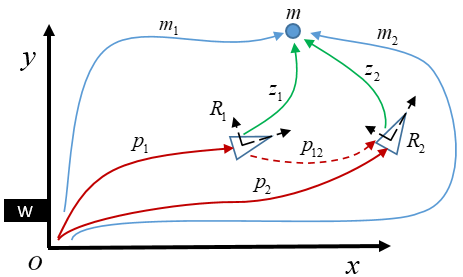
\includegraphics{images/assignment_4.png}
\caption{Example of a possible result}
\end{figure}
Fig 6. Illustration of the scenario in assignment 4.

Consider the following:

\begin{itemize}
\tightlist
\item
  The range-bearing model for taking measurements is \emph{(Note: use
  \href{https://numpy.org/doc/stable/reference/generated/numpy.arctan2.html}{\texttt{np.arctan2()}}
  for computing the angle. At this point, ignore the noise \(w_i\))}:
\end{itemize}

\[
 z_i = \begin{bmatrix} r_i \\ \alpha_i \end{bmatrix} = h(x,m_i) + w_i = 
 \begin{bmatrix} \sqrt((x_i-x)^2+(y_i-y)^2) \\ atan(\frac{y_i-y}{x_i-x}) - \theta \end{bmatrix} 
 + w_i
 \] \(\\[5pt]\)

\begin{itemize}
\item
  We need to compute the covariance of the predicted observation in
  Polar coordinates \((W_{2p})\). For that, use the following:
  \(\\[10pt]\)

  \[ W_{z2\_c} = \frac{\partial f(p2,z_{1\_w})}{\partial \ominus p2} \frac{\ominus p2}{\partial p2} \ Q_{p2\_w} \ \frac{\ominus p2}{\partial p2}^T \ \left( \frac{\partial f(p2,z_{1\_w})}{\partial p} \right)^T +
       \frac{\partial f(p2,z_{1\_w})}{\partial z_{1\_w}} \ W_{z_1\_w} \ \left( \frac{\partial f(p2,z_{1\_w})}{\partial z_{1\_w}} \right)^T
  \]

  \$\$ \text{Applying the Chain rule} \rightarrow W\_\{z2\_c\} =
  \frac{\partial f(p2,z_{1\_w})}{\partial \ominus p2}
  \Sigma\_\{\ominus p2\}
  \frac{\partial f(p2,z_{1\_w})}{\partial \ominus p2}\^{}T
\item
  \frac{\partial f(p2,z_{1\_w})}{\partial p2} ~W\_\{z\_1\_w\}
  ~\frac{\partial f(p2,z_{1\_w})}{\partial p2}\^{}T \$\$
\end{itemize}

Once you have the covariance expressed in cartesian coordinates, you can
express it in polars by means of the following Jacobian:

\[
     \frac{\partial{p}}{\partial{c}} = 
     \begin{bmatrix}
         \cos{(\alpha+\theta)}  & \sin{(\alpha+\theta)} \\
         -\sin{(\alpha+\theta)} / r  & \cos{(\alpha+\theta)} / r
     \end{bmatrix}
 \]

    \begin{tcolorbox}[breakable, size=fbox, boxrule=1pt, pad at break*=1mm,colback=cellbackground, colframe=cellborder]
\prompt{In}{incolor}{8}{\boxspacing}
\begin{Verbatim}[commandchars=\\\{\}]
\PY{k}{def} \PY{n+nf}{predicted\PYZus{}obs\PYZus{}from\PYZus{}pov}\PY{p}{(}\PY{n}{p1\PYZus{}w}\PY{p}{,} \PY{n}{Qp1\PYZus{}w}\PY{p}{,} \PY{n}{z1\PYZus{}w}\PY{p}{,} \PY{n}{Wz1\PYZus{}w}\PY{p}{)}\PY{p}{:}
    \PY{l+s+sd}{\PYZdq{}\PYZdq{}\PYZdq{} Method to translate a pose+covariance in the world frame to an observation.}
\PY{l+s+sd}{    }
\PY{l+s+sd}{        This method only translated the landmark to the pov of the robot.}
\PY{l+s+sd}{        It does not simulate a new observation.}
\PY{l+s+sd}{        }
\PY{l+s+sd}{        Args:}
\PY{l+s+sd}{            p1\PYZus{}w: Pose of the robot which acts as pov}
\PY{l+s+sd}{            z1\PYZus{}w: Landmark observed in cartesian coordinates(world frame)}
\PY{l+s+sd}{            Wz1\PYZus{}w: Covariance associated to the landmark.}
\PY{l+s+sd}{        Returns:}
\PY{l+s+sd}{            z2\PYZus{}pr: Expected observation of z1 from pov of p1\PYZus{}w}
\PY{l+s+sd}{            W2\PYZus{}p: Covariance associated to z2\PYZus{}pr}
\PY{l+s+sd}{    \PYZdq{}\PYZdq{}\PYZdq{}}

    \PY{c+c1}{\PYZsh{} Take a measurement using the range\PYZhy{}bearing model}
    \PY{n}{z2\PYZus{}pr} \PY{o}{=} \PY{n}{np}\PY{o}{.}\PY{n}{vstack}\PY{p}{(}\PY{p}{[}
            \PY{n}{np}\PY{o}{.}\PY{n}{sqrt}\PY{p}{(} \PY{p}{(}\PY{n}{z1\PYZus{}w}\PY{p}{[}\PY{l+m+mi}{0}\PY{p}{]}\PY{o}{\PYZhy{}}\PY{n}{p1\PYZus{}w}\PY{p}{[}\PY{l+m+mi}{0}\PY{p}{]}\PY{p}{)}\PY{o}{*}\PY{o}{*}\PY{l+m+mi}{2} \PY{o}{+} \PY{p}{(}\PY{n}{z1\PYZus{}w}\PY{p}{[}\PY{l+m+mi}{1}\PY{p}{]}\PY{o}{\PYZhy{}}\PY{n}{p1\PYZus{}w}\PY{p}{[}\PY{l+m+mi}{1}\PY{p}{]}\PY{p}{)}\PY{o}{*}\PY{o}{*}\PY{l+m+mi}{2} \PY{p}{)}\PY{p}{,} \PY{c+c1}{\PYZsh{} distance}
            \PY{n}{np}\PY{o}{.}\PY{n}{arctan2}\PY{p}{(} \PY{p}{(}\PY{n}{z1\PYZus{}w}\PY{p}{[}\PY{l+m+mi}{1}\PY{p}{]}\PY{o}{\PYZhy{}}\PY{n}{p1\PYZus{}w}\PY{p}{[}\PY{l+m+mi}{1}\PY{p}{]}\PY{p}{)}\PY{p}{,} \PY{p}{(}\PY{n}{z1\PYZus{}w}\PY{p}{[}\PY{l+m+mi}{0}\PY{p}{]}\PY{o}{\PYZhy{}}\PY{n}{p1\PYZus{}w}\PY{p}{[}\PY{l+m+mi}{0}\PY{p}{]}\PY{p}{)} \PY{p}{)} \PY{o}{\PYZhy{}} \PY{n}{p1\PYZus{}w}\PY{p}{[}\PY{l+m+mi}{2}\PY{p}{]} \PY{c+c1}{\PYZsh{} angle}
        \PY{p}{]}\PY{p}{)}
    
    \PY{c+c1}{\PYZsh{} Obtain the uncertainty in the R2 reference frame using the composition of a pose and a landmark: }
    \PY{n}{z1\PYZus{}ext} \PY{o}{=} \PY{n}{np}\PY{o}{.}\PY{n}{vstack}\PY{p}{(}\PY{p}{[}\PY{n}{z1\PYZus{}w}\PY{p}{,} \PY{l+m+mi}{0}\PY{p}{]}\PY{p}{)} \PY{c+c1}{\PYZsh{} Prepare position and uncertainty shapes to the ones expected by inverse\PYZus{}composition}
    \PY{n}{Wz1\PYZus{}w\PYZus{}ext} \PY{o}{=} \PY{n}{np}\PY{o}{.}\PY{n}{pad}\PY{p}{(}\PY{n}{Wz1\PYZus{}w}\PY{p}{,} \PY{p}{[}\PY{p}{(}\PY{l+m+mi}{0}\PY{p}{,} \PY{l+m+mi}{1}\PY{p}{)}\PY{p}{,} \PY{p}{(}\PY{l+m+mi}{0}\PY{p}{,} \PY{l+m+mi}{1}\PY{p}{)}\PY{p}{]}\PY{p}{,} \PY{n}{mode}\PY{o}{=}\PY{l+s+s1}{\PYZsq{}}\PY{l+s+s1}{constant}\PY{l+s+s1}{\PYZsq{}}\PY{p}{)}
    
    \PY{n}{\PYZus{}}\PY{p}{,} \PY{n}{Wz1\PYZus{}r} \PY{o}{=} \PY{n}{inverse\PYZus{}composition1}\PY{p}{(}\PY{n}{p1\PYZus{}w}\PY{p}{,} \PY{n}{Qp1\PYZus{}w}\PY{p}{,} \PY{n}{z1\PYZus{}ext}\PY{p}{,} \PY{n}{Wz1\PYZus{}w\PYZus{}ext}\PY{p}{)}
        
    \PY{n}{W2\PYZus{}c} \PY{o}{=} \PY{n}{Wz1\PYZus{}r}\PY{p}{[}\PY{l+m+mi}{0}\PY{p}{:}\PY{l+m+mi}{2}\PY{p}{,}\PY{p}{:}\PY{p}{]}
    
    \PY{c+c1}{\PYZsh{} Jacobian from cartesian to polar at z2p\PYZus{}r}
    \PY{n}{theta} \PY{o}{=} \PY{n}{z2\PYZus{}pr}\PY{p}{[}\PY{l+m+mi}{1}\PY{p}{,} \PY{l+m+mi}{0}\PY{p}{]} \PY{o}{+} \PY{n}{p1\PYZus{}w}\PY{p}{[}\PY{l+m+mi}{2}\PY{p}{,} \PY{l+m+mi}{0}\PY{p}{]} 
    \PY{n}{s}\PY{p}{,} \PY{n}{c} \PY{o}{=} \PY{n}{np}\PY{o}{.}\PY{n}{sin}\PY{p}{(}\PY{n}{theta}\PY{p}{)}\PY{p}{,} \PY{n}{np}\PY{o}{.}\PY{n}{cos}\PY{p}{(}\PY{n}{theta}\PY{p}{)}
    \PY{n}{r} \PY{o}{=} \PY{n}{z2\PYZus{}pr}\PY{p}{[}\PY{l+m+mi}{0}\PY{p}{,} \PY{l+m+mi}{0}\PY{p}{]}
    
    
    \PY{n}{Jac\PYZus{}car\PYZus{}pol} \PY{o}{=} \PY{n}{np}\PY{o}{.}\PY{n}{array}\PY{p}{(}\PY{p}{[}
        \PY{p}{[}\PY{n}{c}\PY{p}{,} \PY{n}{s}\PY{p}{]}\PY{p}{,}
        \PY{p}{[}\PY{o}{\PYZhy{}}\PY{n}{s}\PY{o}{/}\PY{n}{r}\PY{p}{,} \PY{n}{c}\PY{o}{/}\PY{n}{r}\PY{p}{]}
    \PY{p}{]}\PY{p}{)}

    \PY{c+c1}{\PYZsh{} Finally, propagate the uncertainty to polar coordinates in the}
    \PY{c+c1}{\PYZsh{} robot frame}
    \PY{n}{W2\PYZus{}p} \PY{o}{=} \PY{n}{Jac\PYZus{}car\PYZus{}pol}\PY{n+nd}{@W2\PYZus{}c}\PY{p}{[}\PY{p}{:}\PY{p}{,}\PY{p}{:}\PY{l+m+mi}{2}\PY{p}{]}\PY{n+nd}{@Jac\PYZus{}car\PYZus{}pol}\PY{o}{.}\PY{n}{T}
    
    \PY{k}{return} \PY{n}{z2\PYZus{}pr}\PY{p}{,} \PY{n}{W2\PYZus{}p}
\end{Verbatim}
\end{tcolorbox}

    \begin{tcolorbox}[breakable, size=fbox, boxrule=1pt, pad at break*=1mm,colback=cellbackground, colframe=cellborder]
\prompt{In}{incolor}{9}{\boxspacing}
\begin{Verbatim}[commandchars=\\\{\}]
\PY{n}{p2\PYZus{}w} \PY{o}{=} \PY{n}{np}\PY{o}{.}\PY{n}{vstack}\PY{p}{(}\PY{p}{[}\PY{l+m+mf}{6.}\PY{p}{,} \PY{l+m+mf}{4.}\PY{p}{,} \PY{l+m+mf}{2.1}\PY{p}{]}\PY{p}{)}
\PY{n}{Qp2\PYZus{}w} \PY{o}{=} \PY{n}{np}\PY{o}{.}\PY{n}{diag}\PY{p}{(}\PY{p}{[}\PY{l+m+mf}{0.20}\PY{p}{,} \PY{l+m+mf}{0.09}\PY{p}{,} \PY{l+m+mf}{0.03}\PY{p}{]}\PY{p}{)}

\PY{n}{z2\PYZus{}pr}\PY{p}{,} \PY{n}{W2\PYZus{}p} \PY{o}{=} \PY{n}{predicted\PYZus{}obs\PYZus{}from\PYZus{}pov}\PY{p}{(}\PY{n}{p2\PYZus{}w}\PY{p}{,} \PY{n}{Qp2\PYZus{}w}\PY{p}{,} \PY{n}{z1\PYZus{}w}\PY{p}{,} \PY{n}{Wz1}\PY{p}{)}
\PY{n+nb}{print}\PY{p}{(} \PY{l+s+s1}{\PYZsq{}}\PY{l+s+s1}{\PYZhy{}\PYZhy{}\PYZhy{}\PYZhy{} Exercise 4.1.4 \PYZhy{}\PYZhy{}\PYZhy{}\PYZhy{}}\PY{l+s+se}{\PYZbs{}n}\PY{l+s+s1}{\PYZsq{}}\PY{o}{+}
    \PY{l+s+s1}{\PYZsq{}}\PY{l+s+s1}{z2p\PYZus{}r = }\PY{l+s+si}{\PYZob{}\PYZcb{}}\PY{l+s+se}{\PYZbs{}\PYZsq{}}\PY{l+s+se}{\PYZbs{}n}\PY{l+s+s1}{\PYZsq{}}\PY{o}{.}\PY{n}{format}\PY{p}{(}\PY{n}{z2\PYZus{}pr}\PY{o}{.}\PY{n}{flatten}\PY{p}{(}\PY{p}{)}\PY{p}{)}\PY{o}{+}
    \PY{l+s+s1}{\PYZsq{}}\PY{l+s+s1}{W2\PYZus{}p = }\PY{l+s+se}{\PYZbs{}n}\PY{l+s+si}{\PYZob{}\PYZcb{}}\PY{l+s+se}{\PYZbs{}n}\PY{l+s+s1}{\PYZsq{}}\PY{o}{.}\PY{n}{format}\PY{p}{(}\PY{n}{W2\PYZus{}p}\PY{p}{)}    
\PY{p}{)}
\end{Verbatim}
\end{tcolorbox}

    \begin{Verbatim}[commandchars=\\\{\}]
---- Exercise 4.1.4 ----
z2p\_r = [3.94880545 0.58862004]'
W2\_p =
[[1.41886714 0.01057848]
 [0.01057848 0.07881227]]

    \end{Verbatim}

    {Expected output:}

\begin{verbatim}
---- Exercise 4.1.4 ----
z2p_r = [3.94880545 0.58862004]'
W2_p = 
[[1.41886714 0.01057848]
 [0.01057848 0.07881227]]
\end{verbatim}

    \hypertarget{assignment-5-combining-observations-of-the-same-landmark}{%
\subsubsection{\texorpdfstring{\textbf{{ASSIGNMENT 5: Combining
observations of the same
landmark}}}{ASSIGNMENT 5: Combining observations of the same landmark}}\label{assignment-5-combining-observations-of-the-same-landmark}}

Assume now that a measurement \(z_2 = [4 m., 0.3 rad.]^T\) of the
landmark is taken from R2 with a sensor having the same precision as
that of R1 (\(W_{2p}= W_{1p}\)). \textbf{You have to}:

\begin{enumerate}
\def\labelenumi{\arabic{enumi}.}
\tightlist
\item
  Use the previously implemented \texttt{to\_world\_frame()} function to
  compute the position and uncertainty about both measurements (\(z1\)
  and \(z2\)) in the world frame.
\item
  Plot the robots and the two measurements along with their uncertainty
  (ellipses) in the world frame.
\item
  Combine both observations within the \texttt{combine\_pdfs()}
  function, and show the resultant combined observation along with its
  associated uncertainty.
\end{enumerate}

\begin{figure}
\centering
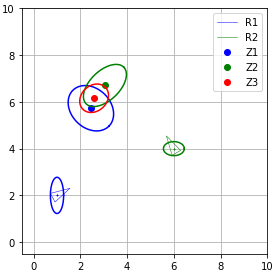
\includegraphics{images/fig4-1-2.png}
\caption{Example of a possible result}
\end{figure}
Fig. 7: Results from the last exercise.

    \begin{tcolorbox}[breakable, size=fbox, boxrule=1pt, pad at break*=1mm,colback=cellbackground, colframe=cellborder]
\prompt{In}{incolor}{10}{\boxspacing}
\begin{Verbatim}[commandchars=\\\{\}]
\PY{k}{def} \PY{n+nf}{combine\PYZus{}pdfs}\PY{p}{(}\PY{n}{z1\PYZus{}w}\PY{p}{,} \PY{n}{Wz1\PYZus{}w}\PY{p}{,} \PY{n}{z2\PYZus{}w}\PY{p}{,} \PY{n}{Wz2\PYZus{}w}\PY{p}{)}\PY{p}{:}
    \PY{l+s+sd}{\PYZdq{}\PYZdq{}\PYZdq{} Method to combine the pdfs associated with two observations of the same landmark.  }
\PY{l+s+sd}{        }
\PY{l+s+sd}{        Args:            }
\PY{l+s+sd}{            z1\PYZus{}w: Landmark observed in cartesian coordinates(world frame) from Robot 1}
\PY{l+s+sd}{            Wz1\PYZus{}w: Covariance associated to the landmark.}
\PY{l+s+sd}{            z1\PYZus{}w: Landmark observed in cartesian coordinates(world frame) from Robot 2}
\PY{l+s+sd}{            Wz2\PYZus{}w: Covariance associated to the landmark.}
\PY{l+s+sd}{        Returns:}
\PY{l+s+sd}{            z: Combined observation}
\PY{l+s+sd}{            W\PYZus{}z: Uncertainty associated to z}
\PY{l+s+sd}{    \PYZdq{}\PYZdq{}\PYZdq{}}
    
    \PY{n}{invs1} \PY{o}{=} \PY{n}{linalg}\PY{o}{.}\PY{n}{inv}\PY{p}{(}\PY{n}{Wz1\PYZus{}w}\PY{p}{)}
    \PY{n}{invs2} \PY{o}{=} \PY{n}{linalg}\PY{o}{.}\PY{n}{inv}\PY{p}{(}\PY{n}{Wz2\PYZus{}w}\PY{p}{)}

    \PY{n}{W\PYZus{}z} \PY{o}{=} \PY{n}{linalg}\PY{o}{.}\PY{n}{inv}\PY{p}{(}\PY{n}{invs1}\PY{o}{+}\PY{n}{invs2}\PY{p}{)}
    \PY{n}{z} \PY{o}{=} \PY{n}{W\PYZus{}z}\PY{o}{@}\PY{p}{(}\PY{p}{(}\PY{n}{invs1}\PY{n+nd}{@z1\PYZus{}w}\PY{p}{)}\PY{o}{+}\PY{p}{(}\PY{n}{invs2}\PY{n+nd}{@z2\PYZus{}w}\PY{p}{)}\PY{p}{)}
    

    \PY{k}{return} \PY{n}{z}\PY{p}{,} \PY{n}{W\PYZus{}z}
    
\end{Verbatim}
\end{tcolorbox}

    \begin{tcolorbox}[breakable, size=fbox, boxrule=1pt, pad at break*=1mm,colback=cellbackground, colframe=cellborder]
\prompt{In}{incolor}{11}{\boxspacing}
\begin{Verbatim}[commandchars=\\\{\}]
\PY{n}{z2\PYZus{}p\PYZus{}r} \PY{o}{=} \PY{n}{np}\PY{o}{.}\PY{n}{vstack}\PY{p}{(}\PY{p}{[}\PY{l+m+mf}{4.}\PY{p}{,} \PY{o}{.}\PY{l+m+mi}{3}\PY{p}{]}\PY{p}{)}
\PY{n}{Wz2\PYZus{}p\PYZus{}r} \PY{o}{=} \PY{n}{np}\PY{o}{.}\PY{n}{diag}\PY{p}{(}\PY{p}{[}\PY{l+m+mf}{0.25}\PY{p}{,} \PY{l+m+mf}{0.04}\PY{p}{]}\PY{p}{)}

\PY{n}{z1\PYZus{}w}\PY{p}{,} \PY{n}{Qz1} \PY{o}{=} \PY{n}{to\PYZus{}world\PYZus{}frame}\PY{p}{(}\PY{n}{p1\PYZus{}w}\PY{p}{,} \PY{n}{Qp1\PYZus{}w}\PY{p}{,} \PY{n}{z1\PYZus{}p\PYZus{}r}\PY{p}{,} \PY{n}{W1}\PY{p}{)}
\PY{n}{z2\PYZus{}w}\PY{p}{,} \PY{n}{Qz2} \PY{o}{=} \PY{n}{to\PYZus{}world\PYZus{}frame}\PY{p}{(}\PY{n}{p2\PYZus{}w}\PY{p}{,} \PY{n}{Qp2\PYZus{}w}\PY{p}{,} \PY{n}{z2\PYZus{}p\PYZus{}r}\PY{p}{,} \PY{n}{W1}\PY{p}{)}

\PY{c+c1}{\PYZsh{} Show results}
\PY{n}{fig}\PY{p}{,} \PY{n}{ax} \PY{o}{=} \PY{n}{plt}\PY{o}{.}\PY{n}{subplots}\PY{p}{(}\PY{p}{)}
\PY{n}{plt}\PY{o}{.}\PY{n}{xlim}\PY{p}{(}\PY{p}{[}\PY{o}{\PYZhy{}}\PY{o}{.}\PY{l+m+mi}{5}\PY{p}{,} \PY{l+m+mi}{10}\PY{p}{]}\PY{p}{)}
\PY{n}{plt}\PY{o}{.}\PY{n}{ylim}\PY{p}{(}\PY{p}{[}\PY{o}{\PYZhy{}}\PY{o}{.}\PY{l+m+mi}{5}\PY{p}{,} \PY{l+m+mi}{10}\PY{p}{]}\PY{p}{)}
\PY{n}{plt}\PY{o}{.}\PY{n}{grid}\PY{p}{(}\PY{p}{)}
\PY{n}{plt}\PY{o}{.}\PY{n}{tight\PYZus{}layout}\PY{p}{(}\PY{p}{)}

\PY{n}{fig}\PY{o}{.}\PY{n}{canvas}\PY{o}{.}\PY{n}{draw}\PY{p}{(}\PY{p}{)}

\PY{n}{DrawRobot}\PY{p}{(}\PY{n}{fig}\PY{p}{,} \PY{n}{ax}\PY{p}{,} \PY{n}{p1\PYZus{}w}\PY{p}{,} \PY{n}{label}\PY{o}{=}\PY{l+s+s1}{\PYZsq{}}\PY{l+s+s1}{R1}\PY{l+s+s1}{\PYZsq{}}\PY{p}{,} \PY{n}{color}\PY{o}{=}\PY{l+s+s1}{\PYZsq{}}\PY{l+s+s1}{blue}\PY{l+s+s1}{\PYZsq{}}\PY{p}{)}
\PY{n}{PlotEllipse}\PY{p}{(}\PY{n}{fig}\PY{p}{,} \PY{n}{ax}\PY{p}{,} \PY{n}{p1\PYZus{}w}\PY{p}{,} \PY{n}{Qp1\PYZus{}w}\PY{p}{,} \PY{n}{color}\PY{o}{=}\PY{l+s+s1}{\PYZsq{}}\PY{l+s+s1}{blue}\PY{l+s+s1}{\PYZsq{}}\PY{p}{)}

\PY{n}{DrawRobot}\PY{p}{(}\PY{n}{fig}\PY{p}{,} \PY{n}{ax}\PY{p}{,} \PY{n}{p2\PYZus{}w}\PY{p}{,} \PY{n}{label}\PY{o}{=}\PY{l+s+s1}{\PYZsq{}}\PY{l+s+s1}{R2}\PY{l+s+s1}{\PYZsq{}}\PY{p}{,} \PY{n}{color}\PY{o}{=}\PY{l+s+s1}{\PYZsq{}}\PY{l+s+s1}{green}\PY{l+s+s1}{\PYZsq{}}\PY{p}{)}
\PY{n}{PlotEllipse}\PY{p}{(}\PY{n}{fig}\PY{p}{,} \PY{n}{ax}\PY{p}{,} \PY{n}{p2\PYZus{}w}\PY{p}{,} \PY{n}{Qp2\PYZus{}w}\PY{p}{,} \PY{n}{color}\PY{o}{=}\PY{l+s+s1}{\PYZsq{}}\PY{l+s+s1}{green}\PY{l+s+s1}{\PYZsq{}}\PY{p}{)}
   
\PY{n}{ax}\PY{o}{.}\PY{n}{plot}\PY{p}{(}\PY{n}{z1\PYZus{}w}\PY{p}{[}\PY{l+m+mi}{0}\PY{p}{,} \PY{l+m+mi}{0}\PY{p}{]}\PY{p}{,} \PY{n}{z1\PYZus{}w}\PY{p}{[}\PY{l+m+mi}{1}\PY{p}{,} \PY{l+m+mi}{0}\PY{p}{]}\PY{p}{,} \PY{l+s+s1}{\PYZsq{}}\PY{l+s+s1}{o}\PY{l+s+s1}{\PYZsq{}}\PY{p}{,} \PY{n}{label}\PY{o}{=}\PY{l+s+s1}{\PYZsq{}}\PY{l+s+s1}{Z1}\PY{l+s+s1}{\PYZsq{}}\PY{p}{,} \PY{n}{color}\PY{o}{=}\PY{l+s+s1}{\PYZsq{}}\PY{l+s+s1}{blue}\PY{l+s+s1}{\PYZsq{}}\PY{p}{)}
\PY{n}{PlotEllipse}\PY{p}{(}\PY{n}{fig}\PY{p}{,} \PY{n}{ax}\PY{p}{,} \PY{n}{z1\PYZus{}w}\PY{p}{,} \PY{n}{Qz1}\PY{p}{,} \PY{n}{color}\PY{o}{=}\PY{l+s+s1}{\PYZsq{}}\PY{l+s+s1}{blue}\PY{l+s+s1}{\PYZsq{}}\PY{p}{)}
          
\PY{n}{ax}\PY{o}{.}\PY{n}{plot}\PY{p}{(}\PY{n}{z2\PYZus{}w}\PY{p}{[}\PY{l+m+mi}{0}\PY{p}{,} \PY{l+m+mi}{0}\PY{p}{]}\PY{p}{,} \PY{n}{z2\PYZus{}w}\PY{p}{[}\PY{l+m+mi}{1}\PY{p}{,} \PY{l+m+mi}{0}\PY{p}{]}\PY{p}{,} \PY{l+s+s1}{\PYZsq{}}\PY{l+s+s1}{o}\PY{l+s+s1}{\PYZsq{}}\PY{p}{,} \PY{n}{label}\PY{o}{=}\PY{l+s+s1}{\PYZsq{}}\PY{l+s+s1}{Z2}\PY{l+s+s1}{\PYZsq{}}\PY{p}{,} \PY{n}{color}\PY{o}{=}\PY{l+s+s1}{\PYZsq{}}\PY{l+s+s1}{green}\PY{l+s+s1}{\PYZsq{}}\PY{p}{)}
\PY{n}{PlotEllipse}\PY{p}{(}\PY{n}{fig}\PY{p}{,} \PY{n}{ax}\PY{p}{,} \PY{n}{z2\PYZus{}w}\PY{p}{,} \PY{n}{Qz2}\PY{p}{,} \PY{n}{color}\PY{o}{=}\PY{l+s+s1}{\PYZsq{}}\PY{l+s+s1}{green}\PY{l+s+s1}{\PYZsq{}}\PY{p}{)}

\PY{n}{z\PYZus{}w}\PY{p}{,} \PY{n}{Wz\PYZus{}w} \PY{o}{=} \PY{n}{combine\PYZus{}pdfs}\PY{p}{(}\PY{n}{z1\PYZus{}w}\PY{p}{,} \PY{n}{Qz1}\PY{p}{,} \PY{n}{z2\PYZus{}w}\PY{p}{,} \PY{n}{Qz2}\PY{p}{)}
\PY{n}{ax}\PY{o}{.}\PY{n}{plot}\PY{p}{(}\PY{n}{z\PYZus{}w}\PY{p}{[}\PY{l+m+mi}{0}\PY{p}{,} \PY{l+m+mi}{0}\PY{p}{]}\PY{p}{,} \PY{n}{z\PYZus{}w}\PY{p}{[}\PY{l+m+mi}{1}\PY{p}{,} \PY{l+m+mi}{0}\PY{p}{]}\PY{p}{,} \PY{l+s+s1}{\PYZsq{}}\PY{l+s+s1}{o}\PY{l+s+s1}{\PYZsq{}}\PY{p}{,} \PY{n}{label}\PY{o}{=}\PY{l+s+s1}{\PYZsq{}}\PY{l+s+s1}{Z3}\PY{l+s+s1}{\PYZsq{}}\PY{p}{,} \PY{n}{color}\PY{o}{=}\PY{l+s+s1}{\PYZsq{}}\PY{l+s+s1}{red}\PY{l+s+s1}{\PYZsq{}}\PY{p}{)}
\PY{n}{PlotEllipse}\PY{p}{(}\PY{n}{fig}\PY{p}{,} \PY{n}{ax}\PY{p}{,} \PY{n}{z\PYZus{}w}\PY{p}{,} \PY{n}{Wz\PYZus{}w}\PY{p}{,} \PY{n}{color}\PY{o}{=}\PY{l+s+s1}{\PYZsq{}}\PY{l+s+s1}{red}\PY{l+s+s1}{\PYZsq{}}\PY{p}{)}
          
\PY{n}{plt}\PY{o}{.}\PY{n}{legend}\PY{p}{(}\PY{p}{)}

\PY{c+c1}{\PYZsh{} Print results}
\PY{n+nb}{print}\PY{p}{(} \PY{l+s+s1}{\PYZsq{}}\PY{l+s+s1}{\PYZhy{}\PYZhy{}\PYZhy{}\PYZhy{}}\PY{l+s+se}{\PYZbs{}t}\PY{l+s+s1}{Exercise 4.1.5}\PY{l+s+se}{\PYZbs{}t}\PY{l+s+s1}{\PYZhy{}\PYZhy{}\PYZhy{}\PYZhy{}}\PY{l+s+se}{\PYZbs{}n}\PY{l+s+s1}{\PYZsq{}}\PY{o}{+}
    \PY{l+s+s1}{\PYZsq{}}\PY{l+s+s1}{z2\PYZus{}w = }\PY{l+s+si}{\PYZob{}\PYZcb{}}\PY{l+s+se}{\PYZbs{}\PYZsq{}}\PY{l+s+se}{\PYZbs{}n}\PY{l+s+s1}{\PYZsq{}}\PY{o}{.}\PY{n}{format}\PY{p}{(}\PY{n}{z2\PYZus{}w}\PY{o}{.}\PY{n}{flatten}\PY{p}{(}\PY{p}{)}\PY{p}{)}\PY{o}{+}
    \PY{l+s+s1}{\PYZsq{}}\PY{l+s+s1}{Qz2 = }\PY{l+s+se}{\PYZbs{}n}\PY{l+s+si}{\PYZob{}\PYZcb{}}\PY{l+s+se}{\PYZbs{}n}\PY{l+s+s1}{\PYZsq{}}\PY{o}{.}\PY{n}{format}\PY{p}{(}\PY{n}{Qz2}\PY{p}{)}
    \PY{p}{)}

\PY{c+c1}{\PYZsh{} Print results}
\PY{n+nb}{print}\PY{p}{(} \PY{l+s+s1}{\PYZsq{}}\PY{l+s+s1}{\PYZhy{}\PYZhy{}\PYZhy{}\PYZhy{}}\PY{l+s+se}{\PYZbs{}t}\PY{l+s+s1}{Exercise 4.1.5 part 2}\PY{l+s+se}{\PYZbs{}t}\PY{l+s+s1}{\PYZhy{}\PYZhy{}\PYZhy{}\PYZhy{}}\PY{l+s+se}{\PYZbs{}n}\PY{l+s+s1}{\PYZsq{}}\PY{o}{+}
    \PY{l+s+s1}{\PYZsq{}}\PY{l+s+s1}{z\PYZus{}w = }\PY{l+s+si}{\PYZob{}\PYZcb{}}\PY{l+s+se}{\PYZbs{}\PYZsq{}}\PY{l+s+se}{\PYZbs{}n}\PY{l+s+s1}{\PYZsq{}}\PY{o}{.}\PY{n}{format}\PY{p}{(}\PY{n}{z\PYZus{}w}\PY{o}{.}\PY{n}{flatten}\PY{p}{(}\PY{p}{)}\PY{p}{)}\PY{o}{+}
    \PY{l+s+s1}{\PYZsq{}}\PY{l+s+s1}{Wz\PYZus{}w = }\PY{l+s+se}{\PYZbs{}n}\PY{l+s+si}{\PYZob{}\PYZcb{}}\PY{l+s+se}{\PYZbs{}n}\PY{l+s+s1}{\PYZsq{}}\PY{o}{.}\PY{n}{format}\PY{p}{(}\PY{n}{Wz\PYZus{}w}\PY{p}{)}
    \PY{p}{)}
\end{Verbatim}
\end{tcolorbox}

    \begin{Verbatim}[commandchars=\\\{\}]
----    Exercise 4.1.5  ----
z2\_w = [3.05042514 6.70185272]'
Qz2 =
[[0.84693794 0.4333316 ]
 [0.4333316  0.81306206]]

----    Exercise 4.1.5 part 2   ----
z\_w = [2.58757252 6.15534036]'
Wz\_w =
[[0.37966125 0.07773125]
 [0.07773125 0.36999739]]

    \end{Verbatim}

    \begin{center}
    \adjustimage{max size={0.9\linewidth}{0.9\paperheight}}{output_24_1.png}
    \end{center}
    { \hspace*{\fill} \\}
    
    {Expected ouputs:}

\hypertarget{sensor-measurement-from-r2}{%
\subsubsection{Sensor measurement from
R2}\label{sensor-measurement-from-r2}}

\begin{verbatim}
z2_w = [3.05042514 6.70185272]'
Qz2 = 
[[0.84693794 0.4333316 ]
 [0.4333316  0.81306206]]
\end{verbatim}

\hypertarget{combined-information}{%
\subsubsection{Combined information}\label{combined-information}}

\begin{verbatim}
---- Exercise 4.1.5 parte 2 ----
z_w = [2.58757252 6.15534036]'
Wz_w = 
[[0.37966125 0.07773125]
 [0.07773125 0.36999739]]
\end{verbatim}

    \hypertarget{thinking-about-it-1}{%
\subsubsection{Thinking about it (1)}\label{thinking-about-it-1}}

Having completed the code above, you will be able to \textbf{answer the
following questions}:

\begin{itemize}
\tightlist
\item
  When working with landmarks, why do we ignore the information
  regarding orientation?
\end{itemize}

Because a landmark is a point, and points don't have any orientation.
Points just have coordenates (in this case X and Y).

\begin{itemize}
\tightlist
\item
  In the two first assignments we computed the covariance matrix of the
  observation \(z_1\) captured by robot \(R1\) in two different cases:
  when the \(R1\) pose was perfectly known, and having some uncertainty
  about it. Which covariance matrix was bigger? Is it bigger than that
  of the robot? Why?
\end{itemize}

The covariance matrix in the Assignment 2 is bigger. Yes, the covariance
matrix is bigger than the covariance matrix of the robot. This is
because we are adding the robot pose uncertainty to the uncertainty of
the measure.

\begin{itemize}
\tightlist
\item
  When predicting an observation of \(m\) from the second robot \(R2\),
  why did we need to use the Jacobian \({\partial{p}}/{\partial{c}}\)?
\end{itemize}

To transform some coordinates that we have from cartesian (world
reference system) to polar (robot reference system)

\begin{itemize}
\tightlist
\item
  In the last assignment we got two different pdf's associated to the
  same landmark. Is that a contradiction? How did you manage two combine
  these two \emph{pieces of information}?
\end{itemize}

It's not a contradiction since although it's true that they use the same
sensor (and therefore the uncertainty of them are the same), the
uncertainties of robot's poses are not the same. This is the reason why
we get different measures.

Because if we multiply two gaussians, the result is a new gaussian, and
if we abstract the meaning of mean, it is a multiplication.


    % Add a bibliography block to the postdoc
    
    
    
\end{document}
